\documentclass[]{book}
\usepackage{lmodern}
\usepackage{amssymb,amsmath}
\usepackage{ifxetex,ifluatex}
\usepackage{fixltx2e} % provides \textsubscript
\ifnum 0\ifxetex 1\fi\ifluatex 1\fi=0 % if pdftex
  \usepackage[T1]{fontenc}
  \usepackage[utf8]{inputenc}
\else % if luatex or xelatex
  \ifxetex
    \usepackage{mathspec}
  \else
    \usepackage{fontspec}
  \fi
  \defaultfontfeatures{Ligatures=TeX,Scale=MatchLowercase}
\fi
% use upquote if available, for straight quotes in verbatim environments
\IfFileExists{upquote.sty}{\usepackage{upquote}}{}
% use microtype if available
\IfFileExists{microtype.sty}{%
\usepackage{microtype}
\UseMicrotypeSet[protrusion]{basicmath} % disable protrusion for tt fonts
}{}
\usepackage{hyperref}
\hypersetup{unicode=true,
            pdftitle={Project Biglife Planning Tool Guide},
            pdfauthor={Project Big Life},
            pdfborder={0 0 0},
            breaklinks=true}
\urlstyle{same}  % don't use monospace font for urls
\usepackage{natbib}
\bibliographystyle{apalike}
\usepackage{longtable,booktabs}
\usepackage{graphicx,grffile}
\makeatletter
\def\maxwidth{\ifdim\Gin@nat@width>\linewidth\linewidth\else\Gin@nat@width\fi}
\def\maxheight{\ifdim\Gin@nat@height>\textheight\textheight\else\Gin@nat@height\fi}
\makeatother
% Scale images if necessary, so that they will not overflow the page
% margins by default, and it is still possible to overwrite the defaults
% using explicit options in \includegraphics[width, height, ...]{}
\setkeys{Gin}{width=\maxwidth,height=\maxheight,keepaspectratio}
\IfFileExists{parskip.sty}{%
\usepackage{parskip}
}{% else
\setlength{\parindent}{0pt}
\setlength{\parskip}{6pt plus 2pt minus 1pt}
}
\setlength{\emergencystretch}{3em}  % prevent overfull lines
\providecommand{\tightlist}{%
  \setlength{\itemsep}{0pt}\setlength{\parskip}{0pt}}
\setcounter{secnumdepth}{5}
% Redefines (sub)paragraphs to behave more like sections
\ifx\paragraph\undefined\else
\let\oldparagraph\paragraph
\renewcommand{\paragraph}[1]{\oldparagraph{#1}\mbox{}}
\fi
\ifx\subparagraph\undefined\else
\let\oldsubparagraph\subparagraph
\renewcommand{\subparagraph}[1]{\oldsubparagraph{#1}\mbox{}}
\fi

%%% Use protect on footnotes to avoid problems with footnotes in titles
\let\rmarkdownfootnote\footnote%
\def\footnote{\protect\rmarkdownfootnote}

%%% Change title format to be more compact
\usepackage{titling}

% Create subtitle command for use in maketitle
\providecommand{\subtitle}[1]{
  \posttitle{
    \begin{center}\large#1\end{center}
    }
}

\setlength{\droptitle}{-2em}

  \title{Project Biglife Planning Tool Guide}
    \pretitle{\vspace{\droptitle}\centering\huge}
  \posttitle{\par}
    \author{Project Big Life}
    \preauthor{\centering\large\emph}
  \postauthor{\par}
      \predate{\centering\large\emph}
  \postdate{\par}
    \date{2019-09-30}

\usepackage{booktabs}
\usepackage{amsthm}
\makeatletter
\def\thm@space@setup{%
  \thm@preskip=8pt plus 2pt minus 4pt
  \thm@postskip=\thm@preskip
}
\makeatother

\begin{document}
\maketitle

{
\setcounter{tocdepth}{1}
\tableofcontents
}
\hypertarget{introduction}{%
\chapter{Introduction}\label{introduction}}

The Project Big Life Planning Tool (\href{http://planning.projectbiglife.ca/}{PBL Planning Tool}) is a web-based application to assess the burden of health behaviours (smoking, diet, physical activity) and the potential health impact of public health preventive strategies in Canada.

The tool was developed in response to requests from public health departments to create, replicate, and update health status reports such as Public Health Ontario's \href{https://www.ices.on.ca/Publications/Atlases-and-Reports/2012/Seven-More-Years}{Seven More Years} report which examined the impact of health behaviours on health outcomes: mortality and life expectancy.

We hope you find the tool helpful for your research and policy planning, including the development and evaluation of population-based health interventions.

\textbf{The tool can help you to:}

\begin{itemize}
\tightlist
\item
  Determine who in the Canadian population is at risk of dying
\item
  Predict the number of new deaths in different Canadian populations
\item
  Determine how much a risk factor contributes to a health outcome
\item
  Assess the health benefits of potential interventions
\end{itemize}

\textbf{Examples questions the tool can answer}

The Project Big Life Planning Tool can answer the following types of questions:

\begin{itemize}
\tightlist
\item
  What is the life expectancy of people in British Columbia across different levels of educational attainment?
\item
  How many deaths would be prevented if people in Ottawa biked as much as people in Copenhagen?
\item
  What is the burden of smoking on life expectancy in Canada?
\item
  How many deaths would be prevented if everyone in Winnipeg increased their daily exercise by 10\%?
\end{itemize}

The tool, which is well-suited to calculate health burdens for a range of social and demographic groups, provides a resource to examine inequities associated with health behaviours.\citep{manuel2018} The ability to examine the impact of different types of preventive scenarios is also supported \&mdash including population strategies that have a small incremental change in health behaviours for a broad target population or high-risk strategies with a larger change in health behaviours that target a smaller number of high-risk people.\citep{PoRTover}

\textbf{How it works}

The wide range of enhanced surveillance applications is made possible through the tool's use of multivariable predictive algorithms. All algorithms used by the planning tool were developed and validated using data routinely collected by Statistics Canada and provincial health agencies, and the algorithms have been published in various journals. More information about the algorithms can be found in the \protect\hyperlink{background}{Background}, \protect\hyperlink{keyconcepts}{Key concepts} and \protect\hyperlink{mport}{Appendices}.

\textbf{Why should I use the tool?}

\begin{itemize}
\item
  It is \textbf{easy} and \textbf{flexible} to use.

  \begin{itemize}
  \tightlist
  \item
    The user only needs to upload their data and choose which calculation to run.
  \item
    It can be used to assess the future risk of a health outcome.
  \item
    It can be used to assess the effectiveness of different intervention scenarios (e.g., policy) on a health outcome.
  \end{itemize}
\item
  It is \textbf{robust} and \textbf{flexible}.

  \begin{itemize}
  \tightlist
  \item
    It can be used to examine health outcomes in a range of social and demographic groups.
  \item
    It generates \textbf{accurate} predictions.
  \item
    The tool's algorithms have been published in peer-review journals, validated in the Canadian population for a wide range of populations, and are publicly available.
  \end{itemize}
\item
  It is \textbf{private}.

  \begin{itemize}
  \tightlist
  \item
    Loaded data remains on your computer and is not uploaded or sent anywhere.
  \end{itemize}
\end{itemize}

\hypertarget{background}{%
\chapter{Background}\label{background}}

The wide range of enhanced surveillance applications is made possible through the tool's multivariable predictive approach. Compared to traditional approaches, the statistical and machine learning algorithms used by the PBL Planning Tool are a more complex approach to measure the burden from health behaviours.\citep{manuel2018} However, the planning tool carries out those complex calculators for you, without the need for statistical software.

Calculations are performed on a population sample of individuals rather than the traditional approach of using aggregated data. The predictive algorithms use the distinct characteristics of each respondent in the database, rather than assuming a person's risk of a health outcome (e.g., death) is the saame for all respondents with the same age and sex.

The algorithms available on the planning tool have been developed and validated using data routinely-collected by Statistics Canada and provincial health agencies. All algorithms have been published in peer-review journals and are \href{https://github.com/Big-Life-Lab/predictive-algorithms}{publicly available}. More information about multivariable predictive risk algorithms can be found in the \protect\hyperlink{keyconcepts}{key concepts} and \protect\hyperlink{mport}{appendices}.

\textbf{Features and contributing}\\
The PBL Planning Tool is currently a pilot project. You can view changes and new features in the website's \href{http://planning.projectbiglife.ca/}{Change Log}.

We welcome suggestions and issues. Please follow this \href{https://github.com/Big-Life-Lab/PBL-Planning-Tool-Guidance/blob/master/contributing/CONTRIBUTING.md}{guide}.

Please tell us if you have scenarios or uses of the planning tool that you want to share with others by commenting on this GitHub \href{https://github.com/Big-Life-Lab/PBL-Planning-Tool-Guidance/issues/9}{issue}.

\textbf{Acknowledgements}

The PBL Planning Tool was developed by the \href{https://www.projectbiglife.ca}{Project Big Life} Team based at the \href{http://www.ohri.ca/home.asp}{Ottawa Hospital} and the \href{https://www.bruyere.org/en/bruyere-research-institute}{Bruyère Research Institute}.

The tool was made in collaboration with \href{https://www.publichealthontario.ca/}{Public Health Ontario}, the \href{https://pophealthanalytics.com/}{Population Health Analytics Lab} at the University of Toronto and \href{http://www.ottawapublichealth.ca/en/index.aspx}{Ottawa Public Health}.

Tool development was supported by the Ontario Ministry of Health and Long-term Care through the Applied Health Research Question program, administered through \href{https://www.ICES.on.ca}{ICES}.

Algorithms used in the planning tool were developed using linked population data housed at \href{https://www.ices.on.ca/}{ICES} and validated at Statistics Canada. All algorithms have been published in peer-review journals. To learn more about the specific algorithms used in the Project Big Life Planning Tool see our \protect\hyperlink{mport}{appendices} to the specific algorithms or \href{https://www.projectbiglife.ca/science}{Project Big Life} website.

\hypertarget{getting-started}{%
\chapter{Getting Started}\label{getting-started}}

To help you get started quickly with Project Big Life's Planning Tool, we built a Tutorial directly onto the web application.

The tutorial takes you through step-by-step how to use Project Big Life's Planning Tool. The tutorial will not explain the \protect\hyperlink{howto}{steps in detail}) nor will it provide terminology \protect\hyperlink{glossary}{glossary} or how the \protect\hyperlink{mport}{tool operates}, but it will give you an understanding of how easy it is to use the Planning Tool!

\textbf{To access the tutorial}, go onto \href{http://planning.projectbiglife.ca/}{Project Big Life's Planning Tool} and click on the Tutorial button in the top right corner!

\begin{center}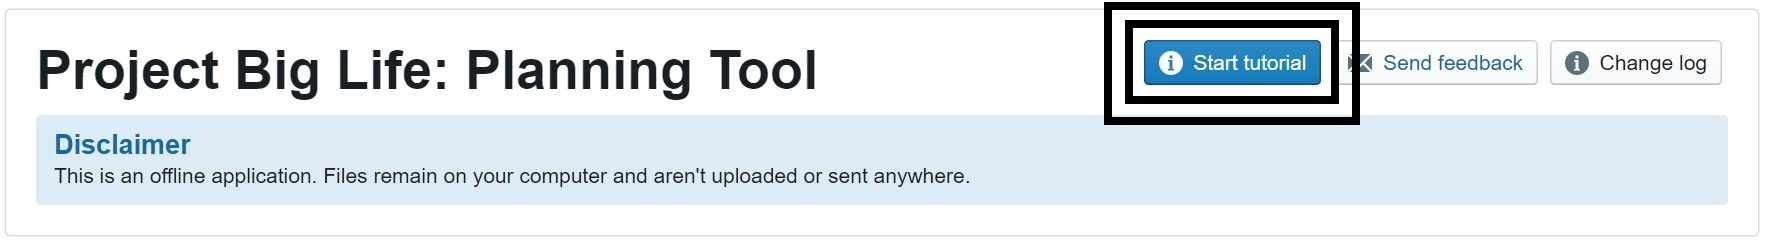
\includegraphics{Images/Tutorial Button} \end{center}

\textbf{Data requirements}
The tool uses the Canadian Community Health Survey (CCHS), Canada's main population health survey administered by Statistics Canada. Information about the CCHS can be found \href{http://www23.statcan.gc.ca/imdb/p2SV.pl?Function=getSurvey\&SDDS=3226}{here}. The tool supports the CCHS 2013 PUMF or Shared files. Information for how to access the CCHS data can be found \href{https://www150.statcan.gc.ca/n1/pub/82-620-m/2005001/4144189-eng.htm}{here}. The Canadian university community can also access the CCCHS through \href{http://odesi2.scholarsportal.info/webview/}{Odesi} -- See health/Canada/Canadian Community Health Survey.

The web application provides two CCHS data samples that can be accessed directly in the web application. These two data samples are synthetic data that do not represent actual respondents. For this reason, the results should not be used other than for demonstration purposes.

\textbf{Web browser support}
The PBL Planning Tool is a web application with all calculations performed on your desktop within the web browswer. Once loaded on your desktop, no connection to the Internet is required.

Please contact the development team if work within a secure research environment without Internet access. We may be able to assist you in creating a broswer-based package that you can transfer onto your internal systems.

\href{mailto:projectbiglife.ca}{projectbiflife@toh.ca} or file an \href{https://github.com/Big-Life-Lab/PBL-Planning-Tool-Guidance/issues}{issue}.

Modern web browsers are supported (Google Chrome, Safari, Firefox, Edge). Internet Explorer is not supported.

\hypertarget{howto}{%
\chapter{How To}\label{howto}}

These guides will cover the topics covered in the tutorial but in greater detail.

\begin{itemize}
\tightlist
\item
  Customize data
\item
  Load data
\item
  Select measure (calculation)
\item
  Filter data
\item
  Stratify data
\item
  Run scenarios: Intervention and Health behaviour attribution
\item
  Calculate results
\item
  Download results (To be developed)
\item
  Resolve error messages (To be developed)
\end{itemize}

\hypertarget{customize-data}{%
\section{Customize Data}\label{customize-data}}

\textbf{Note:} The Project Big Life Planning Tool can only be used with the 2013/2014 Canadian Community Health Survey (CCHS) Public Use Microdata File (PUMF) or Shared versions in `.csv' format.

Other population health surveys can be used only if the required variables are transformed to the specifications of the 2013/2014 CCHS data. Please note that the Project Big Life team is in the process of supporting CCHS versions from 2001 to 2013.

Prior to using the Project Big Life Planning Tool you may want to transform your data set. Reasons include: customized filter(s) and/or customized stratification(s), and transforming variables from other population health surveys to the 2013/2014 Canadian Community Health Survey (CCHS) format. Any variable that you create can be selected within the planning tool in the filter and/or stratify options.

Data manipulation can occur on any programming software: R, SAS, STATA, etc, as long as you output your data set as a `.csv' file.

\hypertarget{customize-filter-andor-stratification}{%
\subsection{Customize filter and/or stratification}\label{customize-filter-andor-stratification}}

An example of customizing your data set is converting the variable: Body Mass Index (CCHS 2013/2014 variable HWTGBMI) from a continuous variable into four distinct categories:

\begin{itemize}
\tightlist
\item
  Underweight: BMI less then 18.5
\item
  Normal or Healthy Weight: BMI of 18.5 to 24.9
\item
  Overweight: BMI of 25.0 to 29.9
\item
  Obese: BMI greater or equal to 30.0
\end{itemize}

\textbf{Steps}

The following steps show the R code that would be used to create these strata:

\begin{enumerate}
\def\labelenumi{\arabic{enumi}.}
\tightlist
\item
  Convert observations ``Not stated'' from 999.99 to NA
\end{enumerate}

\begin{verbatim}
    data[data == 999.99] <- NA
\end{verbatim}

\begin{enumerate}
\def\labelenumi{\arabic{enumi}.}
\setcounter{enumi}{1}
\tightlist
\item
  Load the R package dpylr. This package is used for data manipulation.
\end{enumerate}

\begin{verbatim}
    library(dpylr)
\end{verbatim}

\begin{enumerate}
\def\labelenumi{\arabic{enumi}.}
\setcounter{enumi}{2}
\tightlist
\item
  Create a new column that contains four categories for BMI
\end{enumerate}

\begin{verbatim}
    data$newcolumn <- cut(data$HWTGBMI, breaks = c(0,18.5,25,30,Inf),  labels=c("Underweight", "Healthy", "Overweight", "Obese")
\end{verbatim}

\begin{enumerate}
\def\labelenumi{\arabic{enumi}.}
\setcounter{enumi}{3}
\tightlist
\item
  The output will be your data set + a new column with the corresponding category (``Underweight'', ``Healthy'', ``Overweight'', ``Obese'') for that individual.
\end{enumerate}

\begin{verbatim}
    HWTGBMI   newcolumn
  1   22.68     Healthy
  2   26.99  Overweight
  3      NA        <NA>
  4   34.44       Obese
  5   23.77     Healthy
  6   17.23 Underweight
\end{verbatim}

This new column can be now be used with the Project Big Life Planning Tool for the purpose of filtering or stratification.

\#\#\#Transforming variables to 2013/2014 CCHS format

Population health surveys other then the 2013/2014 CCHS PUMF or Shared files can be used if the variables: sex, age and survey weight (required variables) are transformed to the 2013/2014 CCHS format.

For example the 2005/2006 CCHS data the age variable is titled DHH\textbf{E}GAGE and in the 2013/2014 CCHS data it is DHHGAGE. Although the variable's name changes the data is captured identically in the 2005/2006 and 2013/2014 surveys. Therefore you can use the 2005/2006 CCHS data if you transform this variable to the 2013/2014 format.

\begin{verbatim}
library(dpylr)

CCHSdata.2005.2006 <- CCHSdata.2005.2006 %>% 
  rename(DHHGAGE = DHHEGAGE)
\end{verbatim}

All required variables \textbf{must} be transformed to the 2013/2014 CCHS format. It is also recommended that you transform the recommend variables as well to increase the accuracy of the prediction(s).

When transforming required or recommended variables pay attention to how the variables are captured. There may be differences limit the ability to use the data set or that will affect your results. For instance from the 2001-2004 CCHS survey there are 15 age categories but from 2005-2013 there are 16 age categories.

\hypertarget{load-data}{%
\section{Load data}\label{load-data}}

\textbf{Note:} The Project Big Life Planning Tool can currently only support .csv data files from the 2013/2014 Canadian Community Health Survey (CCHS). Both the 2013/2014 CCHS PUMF and Shared file are accepted.

Data loaded to the Project Big Life Planning Tool:

\begin{itemize}
\item
  \textbf{Must include all} the \textbf{required} variables: DDH\_SEX (sex), DHHGAGE (age), and WTS\_M (survey weight).
\item
  \textbf{Should include} some or all of the \textbf{recommended} variables. Recommended variables aren't required for calculations but will increase the accuracy of the predicted health outcome.
\end{itemize}

More information on the required and recommended variables can be found \protect\hyperlink{mport}{Appendix}.

Only \textbf{one data file} can be used on the planning tool at a time; the planning tool cannot preform a calculation across multiple data files. If you wish to use data from different data sets, you first merge the data sets together and use the 2013/2014 CCHS format (e.g.~variable names). Once data sets are merged into one data file you can load your data on to the Planning Tool.

\textbf{Note:} Data you load to the Project Big Life Planning Tool remains on your computer and is not uploaded or sent anywhere.

There are two options of data files: a sample file or your own file.

\hypertarget{load-sample-files}{%
\subsection{Load sample files}\label{load-sample-files}}

If you don't have your own data or want to explore the platform's capabilities before using your data, you can use the sample file on the Project Big Life Planning Tool. There are two sample files included on the planning tool:

\begin{itemize}
\tightlist
\item
  \textbf{sample.csv (Sample)} this is fabricated data set that includes all variables required for calculation, recommend for calculation, and needed for the \protect\hyperlink{caseexamples}{case examples}. This data set is based on the 2013/2014 CCHS PUMF but it is \textbf{entirely fabricated and can only be used for examplary purposes.}
\item
  \textbf{sample\_small.csv (Sample)} is the same data set as above but has fewer observations. Use this data set if you are testing out the platform as it will take less time to compute.
\end{itemize}

\textbf{Steps}

\begin{enumerate}
\def\labelenumi{\arabic{enumi}.}
\tightlist
\item
  Click on the checkmark beside the ``Sample file'' to select it.
\end{enumerate}

\hypertarget{load-your-own-file}{%
\subsection{Load your own file}\label{load-your-own-file}}

\textbf{Steps}

\begin{enumerate}
\def\labelenumi{\arabic{enumi}.}
\item
  Click the \textbf{Browse} button under ``Select a file to use in calculations''.
\item
  Locate the file on your computer, select, and open.
\item
  Choose the file type (2013/2014 PUMF or 2013/2014 Shared) for your uploaded file, in the table that showcases all of the files.
\end{enumerate}

Note:

\begin{itemize}
\item
  If the loaded file has all of the variables required and recommended for calculation, you will be able to continue with the planning tool.
\item
  If the loaded file does \textbf{not} have all the variables \textbf{required} for the calculation you will not be able to continue with the planning tool.
\item
  If the loaded file does \textbf{not} have all the variables \textbf{recommended} for calculation you will be able to continue with the planning tool, however the calculations may be less accurate.
\end{itemize}

\hypertarget{select-measure-calculation}{%
\section{Select measure (calculation)}\label{select-measure-calculation}}

There are two general types of calculations: summary measures and by row measures.

\begin{itemize}
\item
  \textbf{Summary measures:} When selected, the result will be a single measure for the entire dataset. For instance when Summary Measure - Life Expectancy (Summary Measure) is selected the result is a single life expectancy at birth for the given for the population.
\item
  \textbf{By row measures:} When selected, the result will be the measurement for each individual (e.g.~row) in the dataset.
\end{itemize}

Summary measures must be selected for calculations that have stratifications, intervention scenarios, and health behaviour attribution scenario.

\textbf{Steps}

\begin{enumerate}
\def\labelenumi{\arabic{enumi}.}
\tightlist
\item
  Check the box beside the calculation's name under ``Calculations'' to select it. A single calculation or multiple calculations may be selected.
\end{enumerate}

\begin{itemize}
\tightlist
\item
  Once selected the name(s) of the calculation(s) will appear to the right of ``Calculations''.
\end{itemize}

More details of what the calculations are and how they are preformed can be found in \protect\hyperlink{keyconcepts}{key concepts} - ``Calculations''.

\hypertarget{filter-data}{%
\section{Filter data}\label{filter-data}}

Use filters when you want to analyze only a subset of your data.

\textbf{Steps}

\begin{enumerate}
\def\labelenumi{\arabic{enumi}.}
\item
  Click on the \textbf{+ New} button under ``Filters''.
\item
  Select the variable that you want to filter on by typing its variable name into the ``search variables'' text bar.
\item
  Filter \textbf{in} the categories/levels within the variable by:
\end{enumerate}

\begin{itemize}
\item
  \textbf{Categorical:} Clicking on the ``Search categories''" text bar. Scroll and select the category you want to \textbf{keep} in your data. Repeat this step to add additional categories.
\item
  \textbf{Continous:} Click the ``cycle button'' found under the variable you have selected. Two new boxes will appear.

  \begin{itemize}
  \tightlist
  \item
    Select the minimum value for your subset data in the box on the left by typing the values or using the arrows.
  \item
    Select the maximum value for your subset data in the box on your right by typing the value or using the arrows.
  \end{itemize}
\end{itemize}

\begin{enumerate}
\def\labelenumi{\arabic{enumi}.}
\setcounter{enumi}{3}
\tightlist
\item
  To add another filter repeat the steps above. A maximum of three filters are recommended to maintain statistical power (added filters reduce sample sizes and reduces statistical power).
\end{enumerate}

\begin{itemize}
\tightlist
\item
  Once selected, the name(s) of the filtered variable(s) will appear to the right of ``Filters''.
\end{itemize}

You are able to filter on all types of variables: required for calculation, recommended for calculation, and ignore variables (includes customized variables).

\hypertarget{remove-a-filter}{%
\subsection{Remove a filter}\label{remove-a-filter}}

\begin{itemize}
\item
  To remove a filter entirely, click on the trash can beside the variable you want to delete.
\item
  To remove a level within a filtered variable - categorical, click on the `x' beside the variable level.
\end{itemize}

\hypertarget{stratify-data}{%
\section{Stratify data}\label{stratify-data}}

Use stratifications when you want to get a result for multiple strata (levels or classes).

A summary measure must be selected for stratifications, as only a summary measure will be outputted for each strata. By row measurements may also be selected but they will not be stratified.

\textbf{Steps}

\begin{enumerate}
\def\labelenumi{\arabic{enumi}.}
\item
  Click the box beside either ``Life Expectancy (Summary)'' or ``Deaths (Five Years)'' under the ``Calculation'' drop down.
\item
  Select the variables you want to stratify on under the "Stratifications'. You are only able to stratify on categorical variables.
\item
  To add another variable for stratification repeat the steps above. A maximum of 3 stratifications are recommended to maintain statistical power (added strata reduce strata sample size and reduces statistical power).
\end{enumerate}

\begin{itemize}
\tightlist
\item
  Once selected, the name(s) of the stratified variable(s) will appear to the right of ``Stratifications''.
\end{itemize}

You are able to stratify on all types of categorical variables: required for calculation, recommended for calculation, and ignore variables (includes customized variables).

\hypertarget{remove-a-stratification}{%
\subsection{Remove a stratification}\label{remove-a-stratification}}

\begin{itemize}
\tightlist
\item
  To remove a stratification variable click on the `x' beside the variable level.
\end{itemize}

\hypertarget{run-scenarios}{%
\section{Run scenarios}\label{run-scenarios}}

Scenarios can be used to predict the health outcomes when unhealthy behaviours:

\begin{itemize}
\tightlist
\item
  are modified in the population: \textbf{Intervention}, or
\item
  were never present in the population: \textbf{health behaviour attribution}
\end{itemize}

Scenarios can be used to inform potential health policies or programs.

\hypertarget{intervention-scenarios}{%
\subsection{Intervention scenarios}\label{intervention-scenarios}}

Interventions provide you with the ability to customize the scenarios. For example you can answer the questions:

\begin{itemize}
\tightlist
\item
  what if we only had 15\% of the population smoked rather then the current 20\%?
\item
  what if everyone increased their physical activity by 10\%?
\item
  what if everyone ate 4 fruit servings each day?
\item
  what if everyone drank 2 fewer drinks per week?
\end{itemize}

These intervention scenarios allow you to predict and compare the effectiveness of policies.

There are 3 types of intervention scenarios that you can select:

\begin{itemize}
\tightlist
\item
  \textbf{Absolute:} each individual in the population \textbf{changes} their health behaviour \textbf{by a value of x}.
\item
  \textbf{Relative:} each individual in the population \textbf{changes} their health behaviour \textbf{by a ratio of y}.
\item
  \textbf{Target:} each individual in the population \textbf{has a set value of z.}
\end{itemize}

More information on the specifics of each type of intervention scenario and how they are calculated can be found in \protect\hyperlink{keyconcepts}{key concepts} - ``Scenarios: Interventions''.

\textbf{Steps}

\begin{enumerate}
\def\labelenumi{\arabic{enumi}.}
\item
  Click the box beside either ``Life Expectancy (Summary)'' under the ``Calculation'' drop down.
\item
  Check the button beside: ``Intervention'' under the ``Scenario'' drop down.
\item
  Click on the health behaviour you want to modify: e.g.~Diet.
\end{enumerate}

\begin{itemize}
\tightlist
\item
  A drop down menu of all the possible variables of that health behaviour you can modify will appear.
\end{itemize}

\begin{enumerate}
\def\labelenumi{\arabic{enumi}.}
\setcounter{enumi}{3}
\tightlist
\item
  Click the box beside the variable you want to modify: e.g.~Daily consumption - fruit - (D).
\end{enumerate}

\begin{itemize}
\tightlist
\item
  A drop down menu of the scenario types: absolute, relative, and target, will appear.
\end{itemize}

\begin{enumerate}
\def\labelenumi{\arabic{enumi}.}
\setcounter{enumi}{4}
\item
  Check the button beside the type of intervention you want to modify: e.g.~Target.
\item
  Use the arrows beside the the text box: ``Decrease by'' or ``Increase by'' to add the value you are modifying: e.g.~The value of 4 is used for the scenario what if everyone ate 4 fruit servings each day?
\end{enumerate}

Multiple health behaviours and variables within the health behaviours can be selected for a single calculation.

\begin{itemize}
\tightlist
\item
  Once selected, the name(s) of the health behaviour(s) that have been selected for the intervention will appear to the right of ``Scenario''.
\end{itemize}

\#\#\#Health behaviour attribution scenarios

Health behaviour attribution scenarios provide you with the ability to see the best case scenario for the population. For example:

\begin{itemize}
\tightlist
\item
  what if no one in the population ever smoked?
\item
  what if everyone in the population met their recommended physical activity levels (3.00 METs/week)?
\end{itemize}

More information on health behaviour attribution calculations and how they are calculated can be found in key concepts{]}(\#keyconcepts) - ``Scenarios: Health behaviour attribution''.

\textbf{Steps}

\begin{enumerate}
\def\labelenumi{\arabic{enumi}.}
\item
  Click the box beside either ``Life Expectancy (Summary)'' under the ``Calculation'' drop down.
\item
  Check the button beside: ``Health behaviour attribution'' under the ``Scenario'' drop down.
\item
  Check the box beside the health behaviour that you want to have a health behaviour attribution calculation.
\end{enumerate}

Multiple health behaviours can be selected for a single calculation.

\#\#Calculate results

\begin{enumerate}
\def\labelenumi{\arabic{enumi}.}
\tightlist
\item
  Name your calculation in the text box: Calculation name.
\end{enumerate}

\begin{itemize}
\tightlist
\item
  Be specific when naming the calculation as it will make it easier to distinguish after running multiple calculations.
\end{itemize}

\textbf{Note:} the larger the data set is the longer the calculations will take. Depending on the size of the data set and the type of calculation being preformed it could take an hour or more.

\begin{enumerate}
\def\labelenumi{\arabic{enumi}.}
\setcounter{enumi}{1}
\item
  Click the ``calculate'' button.
\item
  A new table will appear under the calculate button. The table includes the status of the calculation, the calculation: name, measures, filters and stratifications that were select.
\end{enumerate}

A green check mark will appear in the status column.

\#\#View Results

\begin{enumerate}
\def\labelenumi{\arabic{enumi}.}
\item
  Click on the calculation name, in the table under the green calculation button.
\item
  There are three tabs for the results:
\end{enumerate}

\begin{itemize}
\item
  \textbf{Overview:} provides a summary of the calculation that was preformed including: measure, filters used, errors, and warnings.
\item
  \textbf{Stratifications:} This will show the results for the measurement you choose to calculate. This screen will either have:

  \begin{itemize}
  \tightlist
  \item
    \textbf{a table} when you stratifications are selected.
  \item
    \textbf{a graph} when stratification are selected. The graph is further described below.
  \end{itemize}
\item
  \textbf{Log:} will give you a summary of the warnings and errors that occurred during the calculation.
\end{itemize}

\#\#\#Graph

The graph produce through plotly is interactive. Hover over the graph to see the results for each strata, exclude strata, download a .png of the graph, and much more.

\#\#Download results

Click on the \textbf{Download results} button under the \textbf{Results} section.

A pop-up will appear.

Select which measures you would like to download.

Select which calculations you'd like to download.

Scroll down in the pop up window and select ``Download File: Your\_file\_and\_calculation\_name''.

Two files will be downloaded.

\begin{itemize}
\tightlist
\item
  \textbf{Text file:} will give you a summary of the calculation preformed.
\item
  \textbf{CSV file:} will provide you a table with the measures you preformed.
\end{itemize}

\#\#Resolve warning or error messages (To be developed)

There are different types of warning and error messages that may appear.

Below describes some of the messages that are likely to occur and steps to resolve them.

\#\#\#Invalid category

\#\#\#Out of range

\#\#\#Not a number

\#\#\#Sample size is too small

\hypertarget{caseexamples}{%
\chapter{Case examples}\label{caseexamples}}

This chapter provides you with examples of how Project Big Life's Planning Tool can be used in your day-to-day operations. The case examples will cover:

Description

Name

Type

Statistics for health status reports

Health status report

Filter,
Stratification,
Scenario - Health behaviour attributable (smoking and diet)

Deaths prevented from increasing cycling infrastructure

Adjusting gears

Filter,
Scenario - Intervention: Absolute (Physical activity)

Impact on life expectancy by modifying all health behaviours

Healthy cities

Filter,
Stratification,
Scenario - Intervention: Target (All)

Impact on life expectancy by increasing cycling rates

Canada bikes like the Dutch

Filter,
Scenario,
Intervention: Absolute (Physical activity)

Prevented deaths from enacting a 2004 smoking by-law

Smoking by-law, Ottawa 2004: retrospective

Transform variables,
Filter,
Scenario - Intervention: Target (Smoking)

\hypertarget{health-status-report}{%
\section{Health Status Report}\label{health-status-report}}

Health status reports are a way to report the health state for a population and the factors that influence a population's health. Information from health status reports are used to inform policy, planning, and resource allocation.

Using the Project Big Life Planning Tool you can replicate or update existing health status reports e.g.~Public Health Ontario's: \href{https://www.ices.on.ca/Publications/Atlases-and-Reports/2012/Seven-More-Years}{Seven More Years Report} or generate a new health status report.

In this example we will show you how to create some health statistics to include in your health report. We will calculate:

\begin{itemize}
\tightlist
\item
  The predicted number of deaths by strata (e.g.~by sex {[}males and females{]})
\item
  The impact of eliminating unhealthy behaviours on life expectancy
\end{itemize}

For this example we will focus on the population of Alberta.

\hypertarget{predicted-number-of-deaths-stratified-by-sex-and-level-of-education}{%
\subsection{Predicted number of deaths stratified by sex and level of education}\label{predicted-number-of-deaths-stratified-by-sex-and-level-of-education}}

By showing the number of deaths by strata, the reader can see the distribution of deaths across specific population characteristics. Any categorical variable can be used for stratification but in this example we will use sex and level of education.

\textbf{Steps}

\begin{enumerate}
\def\labelenumi{\arabic{enumi}.}
\tightlist
\item
  Select the sample file data.sample.csv under ``Sample files''.
\end{enumerate}

\textbf{Note:} Although the data.sample.csv is based on the 2013/2014 Canadian Community Health Survey Public Use Microdata File, data.sample.csv is a completely synthetic data set and can only be used for exemplary purposes.

\begin{enumerate}
\def\labelenumi{\arabic{enumi}.}
\setcounter{enumi}{1}
\item
  Select the calculation: Summary Measure -- Deaths (Five years)
\item
  Add filter: GEOGPRV -- 48, which is the corresponding code for Alberta.
\item
  Add two stratification: DDH\_SEX and EDUDR04
\item
  Title the calculation: Deaths by sex and education level
\item
  Click the calculate button
\end{enumerate}

\emph{7. To do: Results -- walk through the results}

\hypertarget{impact-of-eliminating-unhealthy-behaviours-smoking-and-poor-diet-on-life-expectancy}{%
\subsection{Impact of eliminating unhealthy behaviours: smoking and poor diet, on life expectancy}\label{impact-of-eliminating-unhealthy-behaviours-smoking-and-poor-diet-on-life-expectancy}}

To show how much an unhealthy behaviour impacts life expectancy we use the scenario: health behaviour attributable. Health behaviour attributable scenarios can be used for the health behaviours: alcohol consumption, diet, physical activity, and smoking, individually or in any combination. In this example we will evaluate the impact of smoking and poor diet, in combination, on life expectancy.

\textbf{Steps}

\begin{enumerate}
\def\labelenumi{\arabic{enumi}.}
\tightlist
\item
  Select the sample file data.sample.csv under ``Sample files''.
\end{enumerate}

\textbf{Note:} Although the data.sample.csv is based on the 2013/2014 Canadian Community Health Survey Public Use Microdata File, data.sample.csv is a completely synthetic data set and can only be used for exemplary purposes.

\begin{enumerate}
\def\labelenumi{\arabic{enumi}.}
\setcounter{enumi}{1}
\item
  Select initial calculation: Summary Measure -- Life Expectancy (Summary)
\item
  Add filter: GEOGPRV -- 48, which is the corresponding code for Alberta.
\item
  Click the text: Scenario.
\item
  Select health behaviour attribution.
\item
  Select the health behaviours: smoking and diet
\item
  Title the calculation: Alberta: smoking and diet attributable life expectancy
\item
  Click the calculate button
\end{enumerate}

\emph{9. To Do: Walk through results}

\textbf{Note:} \(\text{Physical inactivity and poor diet attributable life expectancy lost} \neq\)
\(\text{Physical inactivity-deleted life expectacny} + \text{Poor diet-deleted life expectancy}\)

as individuals in the population may be both physically inactive and have a poor diet.

\hypertarget{adjusting-gears}{%
\section{Adjusting gears}\label{adjusting-gears}}

The City of Hamilton has decided to implement a new initiative \emph{Adjusting Gears} which will increase cycling infrastructure in Hamilton. As part of the plan they have decide to develop 100 km of new cycling infrastructure in the next 3 years (2019-2021).

The city has asked you to evaluate the health impact of this initiative.

As part of the analysis you want to determine how the 100km of new cycling infrastructure will impact the health of the Hamilton area, and how many deaths will be prevented.

\hypertarget{part-a-determine-the-how-much-a-hamiltonian-will-increase-their-physical-activity-by-using-these-new-cycling-tracks}{%
\subsection{Part A: Determine the how much a Hamiltonian will increase their physical activity by using these new cycling tracks}\label{part-a-determine-the-how-much-a-hamiltonian-will-increase-their-physical-activity-by-using-these-new-cycling-tracks}}

Assumption \#1: After having done your research, you assume that with the new tracks the average person in Hamilton will cycle an additional 10 minutes/day (duration).

\begin{enumerate}
\def\labelenumi{\arabic{enumi}.}
\tightlist
\item
  Convert the increased duration of cycling into daily energy expenditure (MET-hours):
\end{enumerate}

\(\text{MET-hours} = \text{Duration}*\text{MET value for cycling}\)

\begin{itemize}
\tightlist
\item
  The MET value for cycling in Canada is 4.0
\end{itemize}

\hypertarget{part-b-determine-the-impact-on-life-expectancy}{%
\subsection{Part B: Determine the impact on life expectancy}\label{part-b-determine-the-impact-on-life-expectancy}}

Use the Project Big Life Planning Tool for the following steps:

\begin{enumerate}
\def\labelenumi{\arabic{enumi}.}
\item
  Load your data file: data.sample.csv to the Project Big Life Planning Tool.
\item
  Select initial calculation: Summary Measure -- Deaths (5-years)
\item
  Add Filter: GEODPMF - 35937
\item
  Click: Scenarios, and select Intervention
\item
  Click Physical Activity then Select ``Average daily leisure time energy expenditure in METs''
\end{enumerate}

Assumption \#2: Although the scenario for physical activity is for leisure energy expenditure, we assume 1) individuals that are active in their leisure time also use active transportation, and 2) cycling as a form of active transportation is minor part of their energy expenditure. Therefore we will adjust the average daily leisure time energy expenditure in METs.

\begin{enumerate}
\def\labelenumi{\arabic{enumi}.}
\setcounter{enumi}{5}
\item
  Select Absolute
\item
  Type in the absolute change calculated in Part 1, into the text box.
\item
  Name your calculation: Adjusting gears - Deaths in Hamilton
\item
  Click Calculate
\end{enumerate}

\hypertarget{healthy-cities}{%
\section{Healthy Cities}\label{healthy-cities}}

What would be Ottawa's life expectancy, if the region had the same health behaviours as the healthiest region in Canada?

In this example, we will determine:

A. who is the healthiest region in Canada,

B. what are the health behaviours of Ottawa vs the healthiest region, and

C. what would be the mortality outcomes be if Ottawa's health behaviours were the same as the healthiest region.

Here we will use the average life expectancy to determine the health of regions: the higher the life expectancy for the region the healthier that region is.

For this example we will use the sample data set \textbf{data.sample.csv}, which can be downloaded at \url{https://github.com/Big-Life-Lab/PBL-Planning-Tool-Case-Examples}. This link also contains all of the R code for this case example. Although we have included the R code any other statistics software (SAS, STATA, etc) can be used to complete this case example.

The following steps include the R coding for each of the steps but you can preform the steps in any other software program.

\hypertarget{part-a-find-the-healthiest-region-in-canada}{%
\subsection{Part A: Find the healthiest region in Canada}\label{part-a-find-the-healthiest-region-in-canada}}

Using the Project Bid Life Planning Tool, we will find the healthiest region in Canada: the region with the highest life expectancy.

\begin{enumerate}
\def\labelenumi{\arabic{enumi}.}
\tightlist
\item
  Load the data file: data.sample.csv.
\end{enumerate}

\textbf{Note:} Although the data.sample.csv is based on the 2013/2014 Canadian Community Health Survey Public Use Microdata File, data.sample.csv is a completely fabricated data set and can only be used for exemplary purposes.

\begin{enumerate}
\def\labelenumi{\arabic{enumi}.}
\setcounter{enumi}{1}
\item
  Select calculation: Summary Measure -- Life Expectancy (Summary)
\item
  Add Stratification: GEODPMF. This variable represents the health regions in Canada
\item
  Title the calculation: Life expectancy by health region
\item
  Click the calculate button
\item
  Download the results - \emph{TO DO}
\end{enumerate}

Using your preferred statistic software (Excel, SAS, STATA, R Studio, etc) identify the healthiest region and the health of the Ottawa health region.

The healthiest region is XXX.

\hypertarget{part-b-determine-the-health-behaviours-of-the-healthiest-region-and-the-ottawa-region.}{%
\subsection{Part B: Determine the health behaviours of the healthiest region and the Ottawa region.}\label{part-b-determine-the-health-behaviours-of-the-healthiest-region-and-the-ottawa-region.}}

Calculate the average of each health behaviour in the healthiest region: XXX and the Ottawa region.

\begin{itemize}
\item
  \textbf{Smoking}: Calculate the prevalence of current smokers in the XXX and Ottawa region.
\item
  \textbf{Physical Activity}: Calculate the average of physical activity (variable PACDEE) in the XXX and Ottawa region.
\item
  \textbf{Alcohol}: Calculate the average of weekly alcohol consumption (variable ALWDWKY) in the XXX and Ottawa region.
\item
  \textbf{Diet}: Calculate the average daily consumption of each diet component (variables: FVCDCAR, FVCDFRU, FVCDJUI, FVCDPOT, FVCDSAL, and FVCDVEG) in the XXX and Ottawa region.

  \begin{itemize}
  \item
    The more daily servings an individual has of:

    \begin{itemize}
    \tightlist
    \item
      carrots, fruits, salad, and vegetables = the more healthy the individual,
    \item
      juice = the less healthy the individual,
    \item
      potato \textless{} 1 = the more healthy the individual, and
    \item
      potato \textgreater{} 1 = the less healthy the individual.
    \end{itemize}
  \end{itemize}
\end{itemize}

\textbf{Comparing health behaviours}

Compare the averages of all health behaviours in the Ottawa region to the XXX. When the health behaviour for Ottawa is unhealthier then XXX, record the avg/prevalence of that health behaviour for XXX.

\hypertarget{part-c-what-if-ottawa-acted-like-xxx}{%
\subsection{Part C: What if Ottawa acted like XXX?}\label{part-c-what-if-ottawa-acted-like-xxx}}

We'll now run a scenario where the Ottawa region acts like XXX. Ottawa will now have the health behaviours of XXX, when the health behaviour of XXX is healthier then Ottawa's.

\begin{enumerate}
\def\labelenumi{\arabic{enumi}.}
\item
  Load your data file: data.sample.csv
\item
  Select initial calculation: Summary Measure -- Life Expectancy (Summary)
\item
  Add Filter: GEODPMF -- 35951 (the code for the Ottawa Health region)
\item
  Click: Scenarios
\item
  Click on each health behaviour where Ottawa is unhealthier then XXX and input XXX's value in the target scenario for that health behaviour
\end{enumerate}

\begin{itemize}
\tightlist
\item
  \emph{TO DO: } Examples of where that is
\end{itemize}

\begin{enumerate}
\def\labelenumi{\arabic{enumi}.}
\setcounter{enumi}{5}
\item
  Title the Calculation: Ottawa - Intervention - HB1, \ldots{}..
\item
  Click calculate.
\item
  \emph{TO DO:} results
\end{enumerate}

\hypertarget{canada-bikes-like-the-dutch}{%
\section{Canada bikes like the Dutch}\label{canada-bikes-like-the-dutch}}

Cycling as a form of transportation, is an effective way of increasing individuals' daily physical activity levels and can lead to a decrease in the risk of disease and death.

In this example we will determine the impact on life expectancy if Canadians were to cycle like the cycling enthusiasts the Dutch!

In this example we determine:

A. How much Canadians cycle per day for transportation purposes on average?

B. How much Dutch cycle per day for transportation purposes on average?

C. What is the average difference in daily cycling transportation for Canadians and the Dutch?

D. Predict how Canadian life expectancy would change if Canadians biked like the Dutch.

For this example we will use the sample data set \textbf{data.sample.csv}, which can be downloaded at \url{https://github.com/Big-Life-Lab/PBL-Planning-Tool-Case-Examples}. This link also contains all of the R code for this case example. Although we have included the Rcode other statistics software (SAS, STATA, etc) can be used to complete this case example.

\textbf{Note:} Although the data.sample.csv is based on the 2013/2014 Canadian Community Health Survey Public Use Microdata File, data.sample.csv is a completely synthetic data set and can only be used for exemplary purposes.

\hypertarget{part-a-how-much-do-canadians-cycle-per-day-for-transportation-purposes-on-average}{%
\subsection{Part A: How much do Canadians cycle per day for transportation purposes on average?}\label{part-a-how-much-do-canadians-cycle-per-day-for-transportation-purposes-on-average}}

We will determine how much Canadians cycle per day by calculating the average daily energy expenditure from cycling in the current Canadian population.

We will use 3 variables in our sample data set which are based off of the 2013/2014 CCHS PUMF and measure cycling as a form of active transportation:

\begin{itemize}
\tightlist
\item
  PAC\_8: In the past 3 months did you cycle to and from work or school?
\item
  PAC\_8A: How many times did you cycle to and from work or school, in the past 3 months?
\item
  PAC\_8B: How much time did you spend on each occasion?
\end{itemize}

\textbf{Assumption \#1:} we assume individuals 65 or older are retired and therefore not cycling to/from work/school. Therefore, we will only evaluate individuals that are \textless{} 65 years old.

In order to calculate the average Canadian daily energy expenditure from cycling for transportation, you will need to:

\begin{itemize}
\item
  Find the average number of times, that an individual cycled to/from work/school in the past 3 months (mean PAC\_8A)
\item
  Find the average number of hours spent cycling to/from work/school, in the past 3 month (mean of PAC\_8B)
\item
  Calculate the average duration of cycling: \(\text{Duration} = [\text{(Frequency/3 months)}*\text{(Time/trip)}] / \text{(Days/3 months)}\)
\item
  Calculate the average daily energy expenditure (MET-hours) for cycling to/from work/school: \(\text{MET-hours} = \text{Duration}*\text{MET value for cycling}\)
\end{itemize}

\textbf{Note:} For Canadians to cycle like the Dutch, we need to use the Dutch MET cycling value of 5.8 and not the Canadian MET cycling value of 4.0. The Dutch MET value accounts for the speed of cycling of the Dutch.

\begin{itemize}
\tightlist
\item
  Calculation the average daily expenditure from cycling for transportation for all individuals in the population not only those that cycled to/from work/school
\end{itemize}

On average a Canadian only gets 0.024 MET-hours/day from cycling to/from work/school.

\hypertarget{part-b-how-much-do-the-dutch-cycleday-for-transportation-purposes-on-average}{%
\subsection{Part B: How much do the Dutch cycle/day for transportation purposes on average?}\label{part-b-how-much-do-the-dutch-cycleday-for-transportation-purposes-on-average}}

Using data collected as part of the Dutch National Travel Survey (2010 -- 2012), Fisherman, 2015 (\url{doi:10.1371/journal.pone.0121871} - Table S1) reported the average additional daily energy expenditure from cycling as a form of transportation for the Dutch: males: 1.3 MET-hours, and females: 1.4 MET-hours.

The average Dutch daily energy expenditure from cycling as a form of transportation for both sexes is then 1.35 MET-hours.

\hypertarget{part-c-what-is-the-average-difference-in-daily-cycling-transporation-for-canadians-and-the-dutch}{%
\subsection{Part C: What is the average difference in daily cycling transporation for Canadians and the Dutch?}\label{part-c-what-is-the-average-difference-in-daily-cycling-transporation-for-canadians-and-the-dutch}}

Canadians need to increase their average daily energy expenditure from cycling from 0.07 MET-hours to 1.35 MET-hours, in order to be like the Dutch.

\textbf{Note:} Since the physical activity intervention scenario on the Project Big Life Planning Tool is for daily leisure energy expenditure and not daily active transportation, we will use the `absolute' scenario for this example. We will increase each individual's daily leisure energy expenditure by 1.28 MET-hours (1.35 MET-hours - 0.07 MET-hours).

\hypertarget{part-d-predict-how-canadian-life-expectancy-would-change-if-canadians-biked-like-the-dutch.}{%
\subsection{Part D: Predict how Canadian life expectancy would change if Canadians biked like the Dutch.}\label{part-d-predict-how-canadian-life-expectancy-would-change-if-canadians-biked-like-the-dutch.}}

Use the Project Big Life Planning Tool for the following steps:

\begin{enumerate}
\def\labelenumi{\arabic{enumi}.}
\item
  Load your data file: data.sample.csv to the Project Big Life Planning Tool.
\item
  Select initial calculation: Summary Measure -- Life Expectancy (Summary)
\item
  Add Filter: DDHGAGE -- 1,2,3,4,5,6,7,8,9,10,11,12
\item
  Click: Scenarios, and select Intervention
\item
  Click Physical Activity then Select ``Average daily leisure time energy expenditure in METs''
\end{enumerate}

Assumption \#2: Although the scenario for physical activity is for leisure energy expenditure, we assume 1) individuals that are active in their leisure time also use active transportation, and 2) cycling as a form of active transportation is minor part of their energy expenditure. Therefore we will adjust the average daily leisure time energy expenditure in METs.

\begin{enumerate}
\def\labelenumi{\arabic{enumi}.}
\setcounter{enumi}{5}
\item
  Select Absolute
\item
  Type in the absolute change calculated in Part 3, into the text box.
\item
  Name your calculation: Canada bikes like the Dutch
\item
  Click Calculate
\item
  Interpret results
\end{enumerate}

\hypertarget{smoking-by-law-2004-ottawa-retrospective}{%
\section{Smoking by-law, 2004 Ottawa: retrospective}\label{smoking-by-law-2004-ottawa-retrospective}}

The City of Ottawa has historically been a leader in municipal policy to reduce tobacco smoking at the population level. A key milestone was the introduction of a 2004 by-law that limited smoking in bars/restaurants.

We want to know how many smoking attributable deaths were prevented due to this by-law.

Assumption: We assume that the by-law lead to decrease in current smokers either through individuals quitting smoking or individuals not starting to smoke.

For this example we will:

A. Transform 2003 CCHS PUMF variables to 2013 CCHS PUMF variables

B. Determine the prevalence of current smokers in 2003

C. Determine the prevalence of current smokers in 2013

D. Estimate how many smoking attributable deaths were prevented due to enacting the by-law

For this example we will use the sample data set \textbf{data.sample2003.csv} and \textbf{data.sample2013.csv}, which can be downloaded at \url{https://github.com/Big-Life-Lab/PBL-Planning-Tool-Case-Examples}. This link also contains all of the R code for this case example. Although we have included the R code any other statistics software (SAS, STATA, etc) can be used to complete this case example.

\hypertarget{part-a-transform-2003-cchs-pumf-variables-to-2013-cchs-pumf-variables}{%
\subsection{Part A: Transform 2003 CCHS PUMF variables to 2013 CCHS PUMF variables}\label{part-a-transform-2003-cchs-pumf-variables-to-2013-cchs-pumf-variables}}

The Project Big Life Planning Tool only works on 2013-2014 CCHS variable names only. Therefore if you are using a CCHS data set from previous years you will have to transform the variables to the 2013-2014 format.

\begin{enumerate}
\def\labelenumi{\arabic{enumi}.}
\tightlist
\item
  Use \textbf{data.sample2003.csv}
\end{enumerate}

\textbf{Note:} Although the data.sample2003.csv is based on the 2003/2004 Canadian Community Health Survey Public Use Microdata File, data.sample2003.csv is a completely fabricated data set and can only be used for exemplary purposes.

With the data.sample2003 data set you will need to:

\begin{itemize}
\item
  Rename 2003 CCHS PUMF variables to their corresponding 2013 CCHS PUMF variables,
\item
  Create variable CCC\_091 from variables CCCC\_91A and CCCC\_91B, and
\item
  Recode DHHGAGE variable
\end{itemize}

Note: The Project Big Life team is developing a R package that will make this step easier for you! The package transforms CCHS variables from 2001 to 2014.

We'll update the guidance as soon as the package is ready!

\hypertarget{part-b-determine-the-prevalence-of-current-smokers-in-2003}{%
\subsection{Part B: Determine the prevalence of current smokers in 2003}\label{part-b-determine-the-prevalence-of-current-smokers-in-2003}}

Current smokers are defined by variable SMKDSTY: 1 -- Daily, 2 -- Occasional, 3 -- Always Occasional.

In 2003, current smokers accounted for 26\% of the Ottawa population.

\#\#\#Part C: Determine the prevalence of current smokers in 2013.

The prevalence of smokers in 2013 will be the scenario target in Part D.

\begin{enumerate}
\def\labelenumi{\arabic{enumi}.}
\tightlist
\item
  Use \textbf{data.sample.csv}
\end{enumerate}

\textbf{Note:} Although the data.sample.csv is based on the 2013/2014 Canadian Community Health Survey Public Use Microdata File, data.sample.csv is a completely fabricated data set and can only be used for exemplary purposes.

In 2013, current smokers accounted for 21\% of the Ottawa population.

\hypertarget{part-d-estimate-how-many-smoking-attributable-deaths-were-prevented-due-to-enacting-the-by-law}{%
\subsection{Part D: Estimate how many smoking attributable deaths were prevented due to enacting the by-law}\label{part-d-estimate-how-many-smoking-attributable-deaths-were-prevented-due-to-enacting-the-by-law}}

Use the Project Big Life Planning Tool for the following steps:

\begin{enumerate}
\def\labelenumi{\arabic{enumi}.}
\item
  Load your data file: data.sample2003.csv to the Project Big Life Planning Tool.
\item
  Select initial calculation: Summary Measure -- Deaths (5 years)
\item
  Add Filter: GEODPMF - 35951
\item
  Click: Scenarios, and select Intervention
\item
  Click Smoking then Select ``Prevalence of current smokers''
\item
  Select Target
\item
  Type in 21 (prevalence of smokers from 2013) into the text box.
\item
  Name your calculation: Smoking attributable deaths 2003
\item
  Click Calculate
\end{enumerate}

\hypertarget{keyconcepts}{%
\chapter{Key Concepts}\label{keyconcepts}}

This section explains some key concepts in Project Big Life's Planning Tool. This section will explain how it works rather then how to do things.

\begin{itemize}
\item
  Data and sample files
\item
  Multivariable predictive risk algorithms
\item
  Calculations: general

  \begin{itemize}
  \tightlist
  \item
    Summary vs.~By Row
  \item
    Weighted vs.~unweighted
  \end{itemize}
\item
  Calculations: specific health outcomes

  \begin{itemize}
  \tightlist
  \item
    Risk of health outcome
  \item
    Number of health outcomes
  \item
    Life expectancy
  \end{itemize}
\item
  Scenario: Intervention
\item
  Scenario: Health behaviour attribution
\item
  Results

  \begin{itemize}
  \tightlist
  \item
    Why are there more deaths for the healthy behaviour?
  \end{itemize}
\item
  Assumptions and limitations
\end{itemize}

\hypertarget{data-and-sample-files}{%
\section{Data and sample files}\label{data-and-sample-files}}

The Project Big Life Planning Tool currently accepts \textbf{2013/2014 Public Use Microdata File and Shared File of the Canadian Community Health Survey (CCHS) in `.csv' format.}

\hypertarget{what-is-the-canadian-community-health-survey}{%
\subsection{What is the Canadian Community Health Survey?}\label{what-is-the-canadian-community-health-survey}}

The CCHS is an annual cross-sectional survey preformed by Statistics Canada. The CCHS collects information related to health status, health care utilization, and health determinants for the Canadian population. Data is shared at the the sub-provincial geographic level (health region or combination of health regions).

\begin{itemize}
\tightlist
\item
  Details about the survey and its design can be found on Statistic Canada website (\url{http://www23.statcan.gc.ca/imdb/p2SV.pl?Function=getSurvey\&Id=144170}).
\item
  Details and access to the Public Use Microdata file (PUMF) can be found through the Odesi website (\url{https://search2.odesi.ca/\#/details?uri=\%2Fodesi\%2Fcchs-82M0013-E-2013-2014-Annual-component.xml})
\end{itemize}

\hypertarget{why-can-the-project-big-life-planning-tool-only-accept-the-20132014-canadian-community-health-survey-data}{%
\subsection{Why can the Project Big Life Planning Tool only accept the 2013/2014 Canadian Community Health Survey data?}\label{why-can-the-project-big-life-planning-tool-only-accept-the-20132014-canadian-community-health-survey-data}}

Each year the CCHS changes a few variables it captures. This makes CCHS data sets from every year other then 2013/2014 partly incompatible with the algorithms used by the Project Big Life Planning Tool.

The Project Big Life Planning Team is currently working to adjust the algorithms so that they accept CCHS year: 2001 to 2014, and will update this guidance.

\hypertarget{can-i-use-other-population-health-survey-data-sets}{%
\subsection{Can I use other population health survey data sets?}\label{can-i-use-other-population-health-survey-data-sets}}

Yes you can use other population health survey data sets but you have to transform these data set to the 2013/2014 CCHS format.

\hypertarget{sample-files}{%
\subsection{Sample Files}\label{sample-files}}

\begin{itemize}
\tightlist
\item
  data.sample.csv this is synthetic data set that includes all variables required for calculation, recommend for calculation, and needed for the case examples (found in Chapter \ref{caseexamples}). While this data set was model on the response rates of the 2013/2014 CCHS PUMF (e.g.~approximately 80\% of respondents did not have high blood pressure (CCC\_071)), the data is fabricated. \textbf{This data set cannot be used for real analysis}.
\end{itemize}

\hypertarget{multivariable-predictive-risk-algorithms}{%
\section{Multivariable predictive risk algorithms}\label{multivariable-predictive-risk-algorithms}}

Multivariable predictive risk algorithms predict the future risk of health outcomes (e.g.~Life Expectancy) for a population using routinely collected health data.

Multivariable predictive risk algorithms can be used to:

\begin{itemize}
\tightlist
\item
  Project the number of new cases of the health outcome
\item
  Estimate the contribution of specific risk factors of the health outcome
\item
  Evaluate effectiveness of health interventions
\item
  Describe the distribution of risk in the population (diffused or concentrated)
\end{itemize}

Multivariable predictive risk algorithms are able to assess equity issues compared to competing population risk methods (e.g.~World Health Organization Global Burden of Disease).

More information on what multivariable predictive risk algorithms are and how they can be used can be found the journal article: \emph{Predictive risk algorithms in a population setting: an overview} \citep{PoRTover}

\hypertarget{development-of-multivariable-predictive-risk-algorithms}{%
\subsection{Development of multivariable predictive risk algorithms}\label{development-of-multivariable-predictive-risk-algorithms}}

Data:

\begin{itemize}
\item
  Multivariable predictive risk algorithms are created using routinely collected data that includes information about risk factors (exposure) and health events (outcomes).
\item
  Data is collected at an individual level through population health surveys (e.g.~Canadian Community Health Survey) and administrative databases (e.g.~Vital Statistics). Data sources are linked together when the individual has given permission too.
\item
  Individuals are followed overtime until the health event (e.g.~death or disease) occurs.
\item
  Separate data is collected to create a derivation cohort and validation cohort(s).

  \begin{itemize}
  \tightlist
  \item
    Note: The risk factors that are collected are from population health surveys and are self-reported; no clinical data (e.g.~blood pressure) is collected. Risk factors focus on health behaviours (e.g.~smoking) and sociodemographic factors, commonly associated with health outcome.
  \end{itemize}
\end{itemize}

\textbf{Algorithm generation:}

\begin{itemize}
\item
  Multivariable predictive risk algorithms are cox proportional hazard models that analyze time to health outcome (e.g.~death) \emph{Question for Carol - The models are not cox-porportional hazard models but they are similar?}
\item
  Multivariable predictive risk algorithms are developed and validated in 4 stages:

  \begin{itemize}
  \tightlist
  \item
    Algorithm derivation: the predictive risk algorithm is created using data from the derivation cohort
  \item
    Algorithm validation: the predictive risk algorithm is applied to the validation cohort
  \item
    Final algorithm generation: validation and derivation cohorts are combined to estimate the final application of the predictive risk algorithm
  \item
    Derivation of the application algorithm: creation of a parsimonous (fewer predictors) algorithm that maintained discrimination, calibration, and overall algorithm performance
  \end{itemize}
\item
  In each stage of the algorithm development and validation, algorithm performance is assessed using measures of discrimination and calibration.
\end{itemize}

\hypertarget{multivariable-predictive-risk-algorithms-built-in-project-big-life-planning-tool}{%
\subsection{Multivariable predictive risk algorithms built in Project Big Life Planning Tool}\label{multivariable-predictive-risk-algorithms-built-in-project-big-life-planning-tool}}

\begin{itemize}
\tightlist
\item
  There is currently 1 multivariable predictive risk algorithm is built into to Project Big Life planning tool.
\end{itemize}

Title

Outcomes

Information

Mortality Population Risk Tool

5 year risk of death, Life Expectancy, Cause deleted

Appendix A

\hypertarget{calculations}{%
\section{Calculations}\label{calculations}}

\hypertarget{summary-vs-by-row}{%
\subsection{Summary vs By Row}\label{summary-vs-by-row}}

There are two general types of calculations Summary Measures and By Row Measures.

Summary measures: When selected, the result will be a single measure for the entire dataset. For instance when Summary Measure - Life Expectancy (Summary Measure) is selected the result is a single life expectancy at birth for the given for the population.

By row measures: When selected, the result will be the measurement for each individual (e.g.~row) in the dataset.

\textbf{Note:} Summary Measures are not the same as taking the average of By Row Measures. Summary measures account for the survey weights in their calculations. Only averaging the By Row Measures does not account for the survey weights and will result in an incorrect outcome.

\hypertarget{weighted-vs-unweighted}{%
\subsection{Weighted vs unweighted}\label{weighted-vs-unweighted}}

Weights are used in complex surveys like the Canadian Community Healthy Survey (CCHS). A weight is given to each respondent in the survey and the weight corresponds to the number of individuals in the population the respondent represents.

When a data set has weights, like the CCHS PUMF data set, the weights are used to calculate the population's outcome e.g.~number of deaths.

When a survey does not have weights, the the population's outcome is not calculated with weights.

In either case, weights are not used in the calculation of an individual's outcome (e.g.~an individual's 5 year risk of mortality).

\hypertarget{calculations-specific-health-outcomes}{%
\section{Calculations: specific health outcomes}\label{calculations-specific-health-outcomes}}

\hypertarget{risk-of-health-outcome}{%
\subsection{Risk of health outcome}\label{risk-of-health-outcome}}

Risk of the health outcome (e.g.~risk of dying) is the outcome of a multivariable predictive risk algorithm. An example of the mutlivariable risk algorithm is:

\[ \text{Risk} = \sum_t h_0(t) * e^{\beta_{pred.smoking}*x_{smoking}+\beta_{pred.cancer}*x_{cancer} + \beta_{pred.age}*x_{age} +...}  \]
Where:

\begin{itemize}
\tightlist
\item
  \(t\) = survival time
\item
  \(h_0(t)\) = the baseline hazard
\item
  \(\beta_{pred}\) = predictive hazard ratios for the exposures
\item
  \(x\) = the exposure. The exposure can be continuous (e.g.~age) or categorical (e.g.~smoking status).
\end{itemize}

Categorical exposures are represented by dummy/factor variables. Each category has its own beta and the exposure is binary. For example smoking status is categorical variable with categories: current, former \textless{}= 5 years, former \textgreater{}5 years, or never smoked. For \(\beta_{pred.current.smoker}\) the exposure: \(x_{current.smoker}\) = 1 if the individual currently smokes or 0 if the individual is another type of smoker.

\hypertarget{number-of-health-outcomes}{%
\subsection{Number of health outcomes}\label{number-of-health-outcomes}}

The number of health outcomes (e.g.~summary - deaths) is calculated through the following steps:

\begin{enumerate}
\def\labelenumi{\arabic{enumi}.}
\item
  Risk of the health outcome is calculated for each individual (row) in the data set using the mutlivariable predictive risk algorithm.
\item
  Each individual's (row) risk is weighted with their corresponding survey weight (CCHS PUMF = WTS\_M and CCHS shared file = WTS\_S).
\item
  The weighted mean of the health outcome (e.g.~mean risk of death) is calculated.
\item
  The weighted mean is then multiplied with the total number of individuals in the population to generate the number of health outcomes (e.g.~number of deaths in 5 years).
\end{enumerate}

\hypertarget{life-expectancy}{%
\subsection{Life expectancy}\label{life-expectancy}}

Life expectancy is calculated using abridge life tables using a modified Chaing approach \citep{Chiang} \citep{Hsieh}. \emph{(link to reference for Chiang and Hsieh and also one of our papers)}. Life expectancy is calculated by two methods: one for summary life expectancy, and a second for by row life expectancy.

\hypertarget{summary-life-expectancy}{%
\subsubsection{Summary Life Expectancy}\label{summary-life-expectancy}}

Life expectancy is calculated separately for males and females.

\textbf{Males:}

\begin{enumerate}
\def\labelenumi{\arabic{enumi}.}
\item
  The mortality risk for each male individual is calculated using the male mortality mutlivariable predictive risk algorithm for mortality (MPoRT). Details about the MPoRT can be found in Appendix A.
\item
  Male individuals are grouped into the 5-year age groups that are used in the 5-year abridge life tables (e.g.~40-44 years old).
\item
  The weighted average risk of death for each age group is calculated.
\item
  A male 5-year abridge life table is created using the weighted average risks of death (q(x)) for each age group and the median age for the age group.
\end{enumerate}

\textbf{Females}

Steps 1-4 used to calculate life expectancy for males, are repeated for females using the female MPoRT and a female 5-year abridge life table.

\textbf{Summary life expectancy}

\begin{enumerate}
\def\labelenumi{\arabic{enumi}.}
\setcounter{enumi}{4}
\tightlist
\item
  The summary life expectancy, or life expectancy of the entire population, is calculated by adding the male life expectancy with the female life expectancy, and taking its average.
\end{enumerate}

\textbf{Summary life expectancy by strata}

Steps (1-4) are repeated for each strata. There will be strata specific weighted risk of death and strata specific life tables.

Step 5 is repeated with the average life expectancy calculated across all strata.

\hypertarget{by-row-life-expectancy}{%
\subsubsection{By row life expectancy}\label{by-row-life-expectancy}}

An individual's life expectancy is calculated by creating a new life table specific to that individual.

These life tables are 1-year abridge life tables, and begin at the individual's age (e.g.~an individual that is 43 years old, will have the life table start at 43 years).

\begin{enumerate}
\def\labelenumi{\arabic{enumi}.}
\item
  The probability of death for a person's current age is calculated using the respective MPoRT (male or female), and the individual's health profile (e.g.~never smoked, 15 drinks weekly, has hypertension, is a Canadian Citizen, etc) (e.g. \(q_x\), where \(x=43\)).
\item
  The probability of death is recalculated for incremental older ages (additional rows of the life table) up to age 90 years ( \(q_\text{(x+1)}, q_\text{(x+2)}...q_{90}\)). For each life table row, age is the only variable that is changed for MPoRT risk calculation.
\end{enumerate}

\textbf{Note:} The result for By Row Life Expectancy are the predicted years of life that the individual still has left to live based on thier age (e.g.~43). To calculate age of death, add the respondent's age to their by row life expectancy estimate.

\textbf{Note:} By row life expectancy does not account for the individual's weight, and therefore can not be used to estimate the summary life expectancy.

\hypertarget{scenario-intervention}{%
\section{Scenario: Intervention}\label{scenario-intervention}}

How would life expectancy change if everyone increased their physical activity levels by 10\%?

The health intervention scenario allows you to predict how changing the health behaviours: alcohol consumption, diet, physical activity, and smoking, of a population will affect the population health outcome (e.g.~life expectancy). This feature can be used to predict the effectiveness of proposed policies or programs.

There are three types of scenarios: \textbf{absolute, relative,} and \textbf{target}.

\begin{itemize}
\tightlist
\item
  \textbf{Absolute:} each individual in the population \textbf{changes} their health behaviour \textbf{by a value of x}.
\item
  \textbf{Relative:} each individual in the population \textbf{changes} their health behaviour \textbf{by a ratio of y}.
\item
  \textbf{Target:} each individual in the population \textbf{has a set value of z.}
\end{itemize}

For target scenarios if the individual's value is already at the target value or beyond the target value then their value is not changed. E.g. If the target value for physical activity is 2.5 METs/day, then any individual that already has METs/day \textgreater{}= 2.5 METs/week then there value will not be adjusted.

The changes for each type of scenario for \textbf{alcohol, physical activity,} and \textbf{diet} are described in the following table:

Health.Behaviour

Absolute.change

Relative.change

Target

Each individual changes \ldots{}

Each individual changes \ldots{}

Each individual has the value \ldots{}

Alcohol Consumption

the number of drinks they have per week by x

the number of drinks they have per week by y \%

z drinks per week

Physical Activity

their physical activity level by x METs per day

their physical activity level by y \% METs per day

z METs per day

Diet

the number of servings of fruits and vegetables they eat by x per day

the number servings of fruits and vegetables they eat by y \% per day

z fruits and vegetables per day

the number of glasses of juice they drink by x per week

the number of glasses of juice by y \% per day

z glasses of juice per day

the number of servings of potatoes the eat by x per week

the number of potatoes they eat by y \% per day

z potatoes per day

The \textbf{smoking} health intervention scenario is different then the other types of health intervention scenarios as they adjust the prevalence of the health behaviour.

Health.Behaviour

Absolute.change

Relative.change

Target

Smoking

The prevalence of smokers decreases by x \%

The prevalence of smokers decreases by y \%

The prevalence of smokers is z \%

Although each type of health intervention for smoking: absolute, relative and target, changes the prevalence of current smokers they are different. The following figure shows how each is different from one another.

\begin{figure}

{\centering 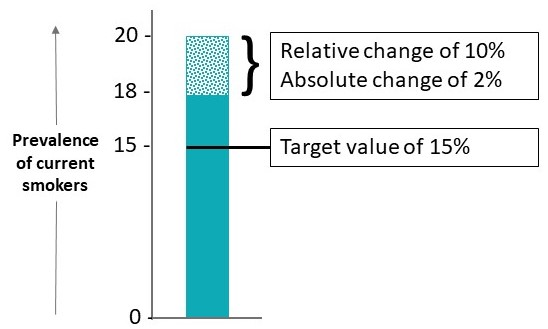
\includegraphics{Images/Scenario-Abs, Rel, Target cropped} 

}

\caption{Comparison of health intervention scenario types}\label{fig:unnamed-chunk-12}
\end{figure}

To adjust the prevalence of smokers, the change is applied to every current smoker in the population; individuals are not selected at random.

\hypertarget{scenario-health-behaviour-attribution}{%
\section{Scenario: Health behaviour attribution}\label{scenario-health-behaviour-attribution}}

What would be the life expectancy of a population if be no one in the population ever smoked? This scenario is a health behaviour attribution scenario.

A health behaviour attribution scenario:

\begin{itemize}
\item
  predicts the health outcome if no one was exposed to the health behaviour = \textbf{health behaviour-deleted outcome}, and
\item
  estimates the effect the health behaviour has on the health outcome for the population = \textbf{health behaviour attributable outcome}
\end{itemize}

To understand health behaviour attribution scenarios lets use the example of smoking and deaths for a population.

The number of deaths for a population is calculated twice:

\begin{itemize}
\tightlist
\item
  with the population that has all smokers = \textbf{baseline deaths}, and
\item
  with a counterfactual scenario where everyone in the population is non-smokers = \textbf{smoking-deleted deaths}
\end{itemize}

The difference between the number of deaths for of the two populations is the \textbf{smoking attributable deaths}.

\begin{figure}

{\centering 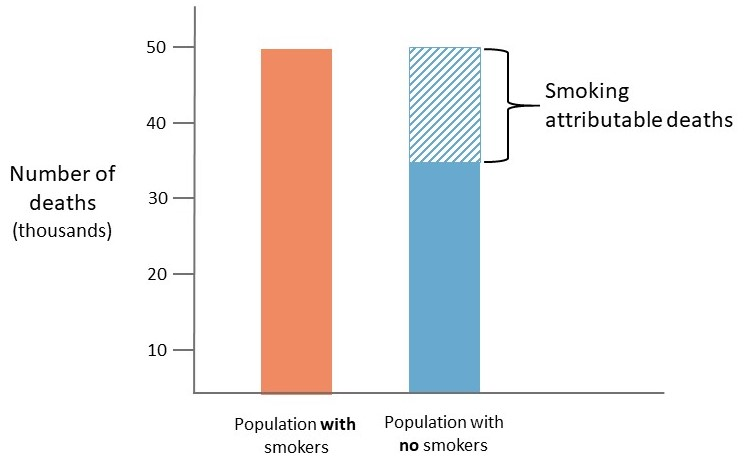
\includegraphics{Images/HB attributable number of deaths} 

}

\caption{Health behaviour attributable scenario - Deaths}\label{fig:unnamed-chunk-13}
\end{figure}

In this example smoking attributes approximately 15,000 deaths in the population.

This can also be done with life expectancy. Life expectancy is calculated:

\begin{itemize}
\tightlist
\item
  with the population that has all smokers = \textbf{baseline life expectancy}, and
\item
  with the counterfactual population where there are no smokers = \textbf{smoking-deleted life expectancy}.
\end{itemize}

The difference between the life expectancy of the two populations is the \textbf{life expectancy lost due to smoking}.

\begin{figure}

{\centering 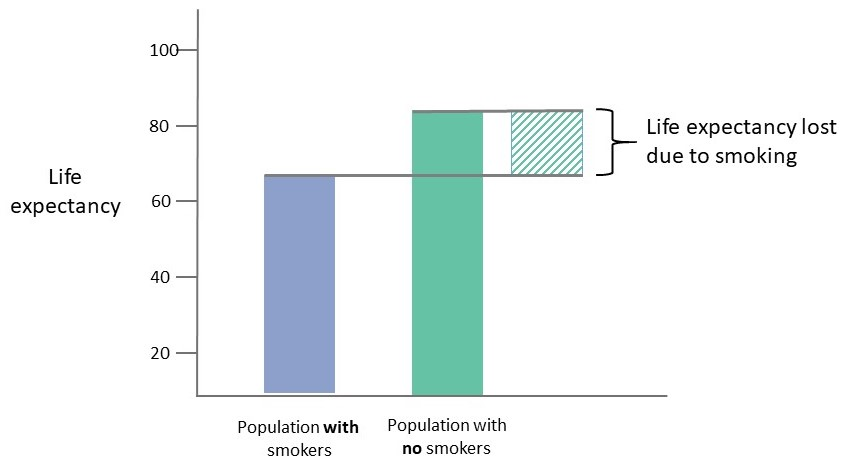
\includegraphics{Images/HB attributable LE} 

}

\caption{Health behaviour attributable scenario - Life expectancy}\label{fig:unnamed-chunk-14}
\end{figure}

\hypertarget{multiple-selected-health-behaviours}{%
\subsection{Multiple selected health behaviours}\label{multiple-selected-health-behaviours}}

If multiple health behaviours are selected the:

\begin{itemize}
\tightlist
\item
  \textbf{health behaviour-deleted outcome} calculated accounts for \textbf{both} of these health behaviours, and
\item
  \textbf{health behaviour attributable outcome} is calculated \textbf{seperately} for each health behaviour.
\end{itemize}

We will use smoking (SMK) and physical inactivity (inPA) to demonstrate what happens when multiple behaviours are selected for health behaviour attribution scenario:

Baseline

Counterfactual

Difference

HealthBehaviour1

HealthBehaviour2

Number of deaths

Deaths

SMK and inPA - deleted deaths

SMK and inPA attributable deaths

SMK attributable deaths

SMK attributable deaths

150,000

100,000

50,000

40,000

15,000

Life expectancy

Life expectancy

SMK and inPA - deleted life expectancy

Life expectancy lost due SMK and inPA

inPA attributable life expectancy lost

inPA attributable life expectancy lost

75

80

5

2

4

\textbf{Note:} \(\text{SMK and inPA - deleted outcome} \neq\)
\(\text{SMK attributable outcome} + \text{inPA attributable outcome}\)

as individuals in the population may be both smokers and physically inactive.

\hypertarget{reference-health-behaviours}{%
\subsection{Reference health behaviours}\label{reference-health-behaviours}}

The health behaviours (references) used to calculate the health behaviour deleted outcomes are:

Health.Behaviour

Reference

Smoking

Never smoker

Alcohol Consumption

0 drinks/week

Physical Activity

3.0 METs/day

Diet

A total of: 5 fruit and vegetables, 0 juice, and 0 potato, servings/day

\hypertarget{results}{%
\section{Results}\label{results}}

\hypertarget{why-are-there-more-deaths-for-the-healthy-behaviour}{%
\subsection{Why are there more deaths for the healthy behaviour?}\label{why-are-there-more-deaths-for-the-healthy-behaviour}}

You may get a result where there are more deaths for the ``healthier'' exposure rather then an ``unhealthier'' exposure, for instance:

\begin{center}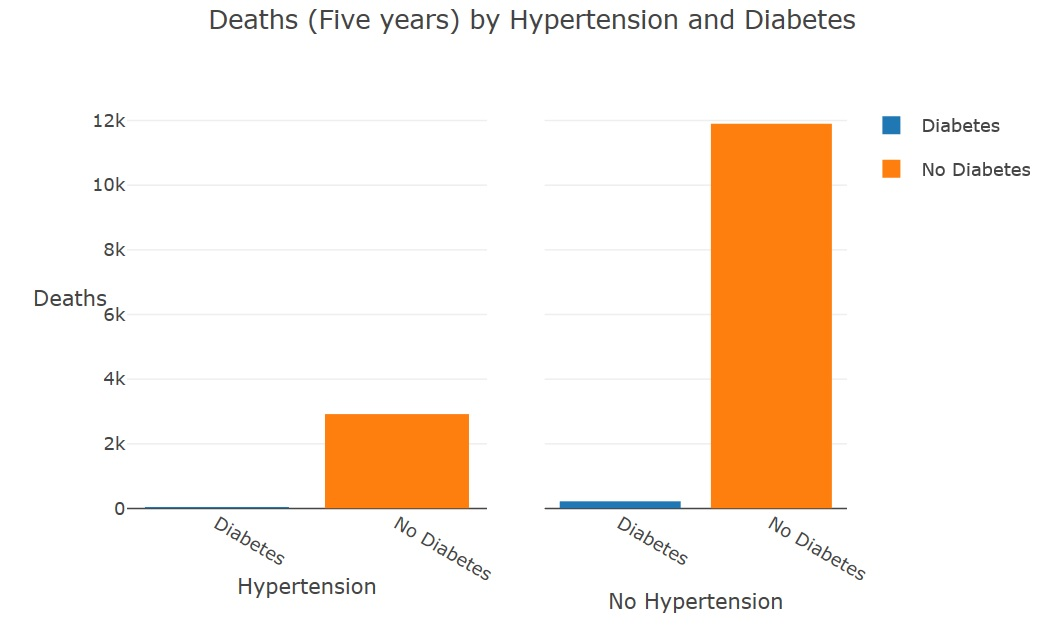
\includegraphics{Images/Graph-hypertension-diabetes} \end{center}

This result occurs as there are more people in the population that do not have diabetes. You can standarized your data set prior to the calculation to get a differnt result.

\hypertarget{assumptions-and-limitations}{%
\section{Assumptions and Limitations}\label{assumptions-and-limitations}}

\hypertarget{limitation-data-source-canadian-community-health-survey}{%
\subsection{Limitation: Data source: Canadian Community Health Survey}\label{limitation-data-source-canadian-community-health-survey}}

\hypertarget{included-population}{%
\subsubsection{Included population}\label{included-population}}

The CCHS survey used to develop the mortality algorithm in the Project Big Life Planning Tool, include only individuals living in the community setting 20 years of age or older. Therefore individuals that live: in long-term care facilities, First Nations reserves, incarcerated populations, and full-time members of the Canadian Forces were excluded.

The exclusion of these individuals is likely to lead to a small under-estimation of the burden of a health behaviour on a health outcome. Excluded populations have higher prevalence of unhealthy behaviours like smoking: incarerated and First Nations have higher prevelance of current smoking and individuals in long-term care facilities are more likely to be former smokers then the general population. However this under-estimation is small as the excluded population only accounts for \textless{} 3\% of the Canadian population.

\hypertarget{reporting-of-health-behaviours}{%
\subsubsection{Reporting of health behaviours}\label{reporting-of-health-behaviours}}

Self-reported data is used to health surveys use self-reported data to predict risk and health outcomes. With self-reported surveys there is the possibility of social desirability bias, where respondents tend to over-report what they perceive to be healthy behaviours and under-report what they perceive to be unhealthy behaviours.

This is particularly the case with alcohol, where there is a consistent under-reporting of alcohol consumption in most population health surveys. In Ontario, the sum of self-reported alcohol consumption is about half the volume of alcohol sold \{\citet{ONalcohol}\}.

In addition the full spectrum of the behaviour has not been captured due to limited questions about the health behaviour in surveys. With diet there were few questions on the CCHS survey and these questions only asked about frequency of diet components. Information on diet factors like quantity, sodium intake, trans fat, or other healthy/unhealthy behaviours were not captured. It is likely that the burden of poor diet is under-estimated.

Although more accurate risk factor ascertainment could improve discriminiation and calibration of the algorithms used in the Project Big Life Planning Tool, these algorithms already have high discrimination and calibration.

\hypertarget{limitation-multivariable-predictive-risk-algorithms}{%
\subsection{Limitation: Multivariable predictive risk algorithms}\label{limitation-multivariable-predictive-risk-algorithms}}

\hypertarget{hazard-ratios-and-exposures-are-assumed-constant}{%
\subsubsection{Hazard ratios and exposures are assumed constant}\label{hazard-ratios-and-exposures-are-assumed-constant}}

The hazard ratios in the algorithms of the Project Big Life Planning Tool, and an individual's exposures are assumed to be constant.

Constant hazard ratios do not account for period effect which could lead to an over-estimation of the burden of a health behaviour e.g.~the differential mortality between smokers and non-smokers may have been greater for older periods, Therefore the algorithms do not account for any period effects.

\hypertarget{limitation-calculations}{%
\subsection{Limitation: Calculations}\label{limitation-calculations}}

\hypertarget{uncertainty}{%
\subsubsection{Uncertainty}\label{uncertainty}}

\hypertarget{attributable-risk-calculations}{%
\subsubsection{Attributable risk calculations}\label{attributable-risk-calculations}}

\hypertarget{limitation-using-the-project-big-life-planning-tool}{%
\subsection{Limitation: Using the Project Big Life Planning Tool}\label{limitation-using-the-project-big-life-planning-tool}}

\hypertarget{glossary}{%
\chapter{Glossary}\label{glossary}}

\textbf{5-year mortality risk}

The probability that an individual will die in the next 5 years.

\textbf{Body Mass Index (BMI)}

A weight-to-height ratio used as an indicator of obesity and underweight. BMI is calculated by dividing an individual's body weight in kilograms by the square of height in metres (kg/m2).

\textbf{By Row Measures}

When selected, the result will be the measurement for each individual (e.g.~row) in the dataset.

\textbf{Calibration}

The agreement between predicted risk generated from the model and observed risk generated from the data.

\textbf{Canadian Community Health Survey}

An annual survey preformed by Statistics Canada that collects information related to health status, health care utilization and health determinants for the Canadian population. Details about the survey can be found on Statistic Canada website (\url{http://www23.statcan.gc.ca/imdb/p2SV.pl?Function=getSurvey\&Id=144170}).

\textbf{Discrimination}

The ability of the model to differentiate between high risk individuals and low risk individuals.

\textbf{Error Message}

Error messages will occur when variables that are \textbf{``Required for Calculation''} are missing in the data. If the entire column for the variable is missing then the calculation cannot be performed on the data. If there are missing row entries for the variable then the entire row will not be used in the calculation.

\textbf{Filter}

Chooses part of your dataset for analysis. If you filter on `Sex' and then `Male', calculations will only be performed on individuals that are `Male' and `Females' will be excluded. For example, when calculating Life Expectancy on the filter variable `Sex' then `Male' there will be a Life Expectancy estimate for `Males' and \emph{no} Life Expectancy estimate for `Females'.

\textbf{Health Behaviour}

Actions people do that may affect their health, positively or negatively. Health behaviours are among the determinants of health and are influenced by the social, cultural and physical environments in which people live and work.\citep{StatsCan2010} They are also shaped by individual choices and external constraints.\citep{StatsCan2010} The four health behaviours of \textbf{smoking, alcohol consumption, diet,} and \textbf{physical activity} are specified in Project Big Life's planning tool.

\textbf{Health behaviour-deleted outcome}

The health behaviour-deleted outcome is the estimated health outcome in a counterfactual population where a specific health behaviour (e.g.~smoking) never existed. For instance, everyone in the counterfactual population were are never smokers.

\textbf{Health behaviour attributable outcome}

The health behaviour attributable outcome represents the effect the health behaviour (e.g.~smoking) has on the health outcome for a population. For example, smoking attributes to 30,000 deaths in the population or 30,000 deaths in the population are caused by smoking.

\textbf{Ignored Variables}

Are not included in the calculation. It does not matter if your dataset includes these variables or not. Ignored variables can used for filter and stratification.

\textbf{Life Expectancy (LE)}

Life expectancy is a calculation of how long a person or population would be expected to live, on average, given unchanging risk of death from a specific point in time.

\textbf{Metabolic Equivalent of Task (MET)}

The metabolic equivalent of task (MET) is a measure of the rate of energy expenditure from an activity; a measure of calories burned by type, duration and frequency of physical activity. The reference value of 1 MET is defined as the energy expediture rate at rest which is equal to 1kcal/kg/day.

\textbf{Predictor}

A variable that is used in the algorithm to predict the outcome.

\textbf{Recommend for calculation}

Variables that are included in the calculation but not necessary for the calculation to run. Rather these variables increase the accuracy of the results.

\textbf{Required for calculation}

Variables that are included in the calculations and are necessary for the calculation to run. If a dataset does not have these variables then the calculation will not run.

\textbf{Risk}

The probability ofa health event occuring at some point of time in the future.

\textbf{Socioeconomic Position}

People in poorer socioeconomic circumstances generally have poorer health. Deprivation measures identify those who experience material or social disadvantage compared to others in their community. The Deprivation Index for Health in Canada developed by the Institut national desanté publique du Québec (INSPQ)\citep{INSPQ2000} is used in this plannning tool. The index includes education, employment and income as measures of material deprivation; and single-parent families, living alone, or being divorced, widowed or separated as measures of social deprivation. The deprivation index was used to assign geographical areas into socioeconomic position groups (low, middle and high) based on material and social quintiles. High-deprivation neighbourhoods were those in the top two quintiles for both social and material deprivation. Low-deprivation neighbourhoods were those in the bottom two quintiles.

\textbf{Stratification}

The seperation of data into smaller strata (levels or classes which individuals are assigned too). If the variable `Sex' is stratified it creates two strata: `Male' and `Female'. Calculations are performed on each strata (level or class) and the outcome will be specific to that strata. For example, when calculating Life Expectancy on the stratified variable `Sex' there will be a Life Expectancy estimate for `Males' and a different Life Expectancy estimate for `Females'.

Stratification can only occur on categorical variables.

\textbf{Summary Measures}

When selected, the result will be a single measure for the entire dataset. For instance when Summary Measure - Life Expectancy (Summary Measure) is selected the result is a single life expectancy at birth for the given for the population.

When stratifications are selected, the summary measure will be given for each strata. For instance when Summary Measure - Life Expectancy and Stratification - Sex are selected, then two life expectancy measures will be given one for males and one for females.

\textbf{Warning Message}

Warning messages will occur when variables that are \textbf{``Recommended for Calculation''} are missing in the data. If the entire column for the variable is missing the calculation will still be performed on the data. If there are missing row entries for the variable the row will still be used in the calculation

\textbf{Weights}

A weight is given to each respondent in the survey and the weight corresponds to the number of individuals in the population the respondent represents.

















\hypertarget{appendix-appendix}{%
\appendix}


\hypertarget{mport}{%
\chapter{Mortality Population Risk Tool (MPoRT)}\label{mport}}

*\textbf{Outcomes: Life Expectancy, Number of deaths, 5-year mortality risk}

\textbf{Calculations}

Using MPoRT you are able to calculate:

\begin{itemize}
\item
  For each individual (By row)

  \begin{itemize}
  \tightlist
  \item
    5 year mortality risk
  \item
    Life Expectancy
  \end{itemize}
\item
  For the population (Summary)

  \begin{itemize}
  \tightlist
  \item
    Number of deaths
  \item
    Life Expectancy
  \item
    Health behaviour-deleted life expectancy
  \item
    Health behaviour-deleted number of deaths
  \item
    Health behaviour attributable life expectancy
  \item
    Health behaviour attributable number of deaths
  \end{itemize}
\end{itemize}

\textbf{Types of Questions}

\begin{itemize}
\tightlist
\item
  What is the burden of smoking on life expectancy?
\item
  How many deaths would be prevented if everyone met their daily exercise requirements?
\end{itemize}

\textbf{Description}

A multivariable predictive risk model that estimates the future risk of all-cause death in Canada. It adjusts for health behaviours: smoking, unhealthy alcohol consumption, poor diet, and physical inactivity, and a wide range of other risk factors.

\hypertarget{data-requirements-for-mport}{%
\section{Data requirements for MPoRT}\label{data-requirements-for-mport}}

In order to use the MPoRT algorithm on the Project Big Life Tool your data set \textbf{must include} the following CCHS 2013/2014 variables:

PUMF\_CCHS\_variable

Shared\_CCHS\_variable

Description

DDH\_SEX

DDH\_SEX

Sex

DHHGAGE*

DHH\_AGE*

Age

WTS\_M*

WTS\_S*

Survey weight

* Variable names are different between the two files

In addition the following variables \textbf{should} be included to increase the prediction accuracy:

PUMF\_CCHS\_variable

Shared\_CCHS\_variable

Description

ALWDWKY

ALWDWKY

Weekly alcohol consumption

CCC\_071

CCC\_071

Do you have high blood pressure

CCC\_091

CCC\_091

Do you have chronic obstructive pulmonary disease

CCC\_101

CCC\_101

Do you have diabetes

CCC\_121

CCC\_121

Do you have heart disease

CCC\_131

CCC\_131

Do you have active cancer

CCC\_151

CCC\_151

Do you suffer from effects of stroke

CCC\_280

CCC\_280

Do you have a mood disorder

EDUDR04

EDUDR04

Highest level/education of respondent

FVCDCAR

FVCDCAR

Daily consumption - carrot

FVCDFRU

FVCDFRU

Daily consumption - fruit

FVCDJUI

FVCDJUI

Daily consumption - juice

FVCDPOT

FVCDPOT

Daily consumption - potatoes

FVCDSAL

FVCDSAL

Daily consumption - green salad

FVCDVEG

FVCDVEG

Daily consumption - vegetables

HWTGBMI*

HWTDBMI*

BMI self reported

PACDEE

PACDEE

Daily energy expenditure

SDCFIMM

SDCFIMM

Immigrant

SDCGCGT*

SDCDCGT*

Cultural or racial origin

SDCGRES*

SDCDRES*

Length of time in Canada since immigration

SMK\_01A

SMK\_01A

In lifetime, smoked 100 or more cigarettes

SMK\_05B

SMK\_05B

\# of cigarettes smoked daily - occasional smoker

SMK\_05C

SMK\_05C

Past month, smoked 1+ cigarettes daily - occasional smoker

SMK\_09A

SMK\_09A

When did you stop smoking daily - occasional smoker

SMK\_204

SMK\_204

\# of cigarettes smoked daily - daily smoker

SMK\_208

SMK\_208

\# of cigarettes smoke each day - occasional smoker

SMKDSTY

SMKDSTY

Type of smoker

SMKG01C*

SMK\_01C*

Age smoked first whole cigarette

SMKG09C*

SMK\_09C*

Years since stopped smoking daily - occasional smoker

SMKG203*

SMK\_203*

Age started to smoke daily

* Variable names are different between the two files

\hypertarget{descriptions-of-mport-versions}{%
\section{Descriptions of MPoRT versions}\label{descriptions-of-mport-versions}}

Versions of MPoRT have been developed since 2012 and used in various studies. Each version of MPoRT (v1.0, v1.2, v2.0) used the Ontario subset of the Canadian Community Health Survey (CCHS) for development and the survey respondents were linked to personal death records. In later versions of MPoRT (v1.2, v2.0) the following changes were made:, (a) algorithm variables were adjusted to improve predictions, and (b) the algorithms were validated using: the Ontario subset of CCHS of the years that were not used in development and the National CCHS data set (excluding Ontario).

\textbf{MPoRTv1.0}

Was used in the \href{https://www.ices.on.ca/Publications/Atlases-and-Reports/2012/Seven-More-Years}{Seven More Years} report, a joint report with Public Health Ontario and ICES .
In summary, the algorithm estimated the risk of death associated with health behaviours: smoking, unhealthy alcohol consumption, poor diet, physical inactivity and stress. There were approximately 550,000 person-years of follow up and over 6000 deaths in the development data set. The algorithm used categorical predictor variables for health behaviours and sociodemographic factors.

\textbf{MPoRTv1.2}

Was published in \href{https://journals.plos.org/plosmedicine/article?id=10.1371/journal.pmed.1002082}{PLoS}.
In summary, the algorithm estimated the risk of death associated with health behaviours: smoking, unhealthy alcohol consumption, poor diet, and physical inactivity (stress was removed due to its low prediction ability). There were approximately 1 million person-years of follow up and over 9000 deaths in the development and validation data sets. The algorithm used multiple continuous predictor variables, and added chronic disease predictor variables and interaction terms.

\textbf{MPoRTv2.0 - Version in Project Big Life's Planning Tool}

This version of MPoRT has not yet been published.

\emph{Development}: This predictive risk model was developed using Ontario subsets of the 2001 to 2008 CCHS and participants were linked to personal health records. There were approximately 1.3 million person-years of follow-up and over 15,000 deaths in the developmental data set.

\emph{Validation}: This predictive risk model was validated using three different data sets: Ontario subset of the 2009 to 2012 CCHS, National data set (except Ontario) of the 2003 to 2008 CCHS, and the National data set of the 2000 and 2005 National Health Interview Survey in the United States of America. In all validation data sets individuals were linked to personal health records.

\emph{Model}: Two MPoRTs have been created: one for males and one for females. Each model is a cox-proportional hazard model that looks similar to:

\[ \text{Mortality risk} = \sum_t h_0(t) * e^{\beta_{pred.smoking}*x_{smoking}+\beta_{pred.cancer}*x_{cancer} + \beta_{pred.age}*x_{age} +...}  \]

Where:

\begin{itemize}
\tightlist
\item
  \(t\) = survival time
\item
  \(h_0(t)\) = the baseline hazard
\item
  \(\beta_{pred}\) = predictive hazard ratios for the exposures
\item
  \(x\) = the exposure. The exposure can be continuous (e.g.~age) or categorical (e.g.~smoking status).
\end{itemize}

\emph{Parameters}: The parameters used in this multivariable predictive risk model are:

Category

Variable

Scale

Description

Demographic

Age*

Continous

5 knot spline. Valid range 20 to 102

Sex

Dichotomous

Stratified Female/Male

Health Behaviour

Pack years of smoking

Continous

3 knot spline. Valid range: 0 to 78 (Female), 0 to 112.5 (Male)

Smoking Status

Categorical

Non-smoker

Current Smoker

Former Smoker \textless{}= 5 years

Former \textgreater{} 5 years

Alcohol (number of drinks per week)

Continous

4 knot spline (Females) and 3 knot spline (Males). Valid range: 0 to 25 (Female), 0 to 50 (Male)

Former/non-drinker

Dichotomous

Yes/No

Simplified diet score

Continous

3 knot spline. Valid range: -18.9 to 20.7 (Female), -16.8 to 18.4 (Male)

Leisure physical activity (MET)

Continous

3 knot spline. Valid range: 0 to 12.4 (Female), 0 to 16 (Male)

Socio-demographic

Ethnicity

Categorical

White

Black

Chinese

Arab; South Asian; West Asian

Filipino; Japanese; Korean; Southeach Asian

Other; Indigenous; Latin American; Multiple origin; unknown

Immigrant

Dichotomous

Yes/No

Fraction of lifetime in Canada

Continous

3 knot spline\textsuperscript{†}. Valid range: 0 to 1

Education

Categorical

Less than secondary

Secondary School Graduation

Some Post-Secondary

Post-Secondary Graduation

Neighbourhood social and material
deprivation

Ordinal

Low (1st or 2nd quantile

High (4th or 5th quantile)

Moderate (all others)

Chronic Conditions

Diabetes

Dichotomous

Yes/No

High Blood Pressure

Dichotomous

Yes/No

Chronic Respiratory Disease

Dichotomous

Yes/No

Mood Disorder

Dichotomous

Yes/No

Cancer

Dichotomous

Yes/No

Dementia

Dichotomous

Yes/No

Heart Disease

Dichotomous

Yes/No

Stroke

Dichotomous

Yes/No

Epilepsy

Dichotomous

Yes/No\textsuperscript{‡}

BMI

Continous

3 knot spline. Valid range: 8.9 to 47.2 (Female), 8.6 to 43.7 (Male)

* Age interaction included for all variables exept immigrant, fraction of time in Canada, and ethnicity † Excluded in the male model, remains in the female model ‡ Excluded in the female model, remains in the male model

\hypertarget{derived-parameters}{%
\subsection{Derived parameters}\label{derived-parameters}}

In MPoRTv2 there are some parameters that are derived from variables within the data set. These include: pack-years of smoking, and the simplified diet score.

\textbf{Pack-years of smoking}

Pack-years of smoking is generated from: the type of smoker, age in which they started smoking daily, how many cigarettes they smoke daily, and if applicable the age in which they stopped smoking daily. Pack-years of smoking also includes: their age, the age of thier first cigarette, and whether throughout thier life they have smoked 100+ cigarettes.

In summary, the more an individual smokes or the longer they smoke, the greater the pack-years of smoking.

\textbf{Simplified Diet Score}

The simplified diet score essentially adds the healthy diet variables together (daily servings of carrots, fruit, salad, vegetables) and subtracts the unhealthy diet variables (daily servings of juice and potato).

\hypertarget{health-behaviour-attributable-calculations}{%
\chapter{Health behaviour attributable calculations}\label{health-behaviour-attributable-calculations}}

Here we will explain the details behind Project Big Life Planning Tool health behaviour attributable scenarios including: the calculations and additional considerations.

\hypertarget{calculation}{%
\section{Calculation}\label{calculation}}

There are two parts to the calculations preformed in health behaviour attributable scenarios: (A) calculate the risk, and (B) calculate the health outcome: life expectancy or number of deaths.

\hypertarget{part-a-risk-calculations}{%
\subsection{Part A: Risk calculations}\label{part-a-risk-calculations}}

The original multivariable predictive risk algorithm is:

\[ \text{Risk} = \sum_t h_0(t) * e^{\beta_{pred.smoking}*x_{smoking}+\beta_{pred.cancer}*x_{cancer} + \beta_{pred.age}*x_{age} +...}  \]

\textbf{Step 1.} Modify the original algorithm to include the external coefficient(s). This means replacing all predictive hazard ratios/betas related to the health behaviour to the causal hazard ratios/betas.

\begin{itemize}
\tightlist
\item
  Remove the original regression coefficient(s) for the health behaviour.
\item
  Add the new external coefficient(s) to the algorithm. External coefficients are generated from either: causal models, or from systematic reviews or meta-analysis.
\end{itemize}

\[ \text{External coefficient risk} = \sum_t h_0(t) * e^{{\beta_\textbf{causal.smoking}}*x_{smoking} + {{\beta_\textbf{causal.cancer}}}*x_{cancer} + \beta_{pred.age}*x_{age} +...}  \]

\textbf{Step 2.} Risk is calculated using the modified algorithm created in Step 1 and the respondent's original profile (e.g.~current smoker). This is the ``external coefficient risk''.

\[ \text{External coefficient risk} = \sum_t h_0(t) * e^{\beta_{causal.smoking}* {(\textbf{current smoker})} + \beta_{causal.cancer}*x_{cancer} + \beta_{pred.age}*x_{age} +...}  \]

\textbf{Step 3.} ``Health behaviour-deleted risk''' is calculated by setting an exposure to a reference (non-exposed) value (all other risk exposures remain unchanged).

\[ \text{Health behaviour-deleted risk' } = \sum_t h_0(t) * e^{\beta_{causal.smoking}* {(\textbf{never smoker})} + \beta_{causal.cancer}*x_{cancer} + \beta_{pred.age}*x_{age} +...}  \]

\textbf{Step 4.} The ``health behaviour attributable risk external'' is calculated as ``external coefficient risk'' (Step 2) minus the ``health behaviour-deleted risk'.''(Step 3).

\[\text{Health behaviour attributable risk}_{external} = \text{External coefficient risk} - \text{Health behaviour-deleted risk'}\]

\textbf{Step 5.} Original risk is calculated using the original algorithm and the original respondent's profile.

\[ \text{Original risk} = \sum_t h_0(t) * e^{{\beta_\textbf{pred.smoking}}*{(\textbf{current smoker})}+{\beta_\textbf{pred.cancer}}*x_{cancer} + \beta_{pred.age}*x_{age} +...}  \]

\textbf{Step 6.} The ``health behaviour-deleted risk external'' is calculated by ``original risk'' (Step 5) minus the ``health behaviour-deleted effect external'' (Step 4).

\[\text{Health behaviour-deleted risk}_{ external} = \text{Original risk} - \text{Health behaviour attributable risk}_{external}\]

\begin{figure}

{\centering 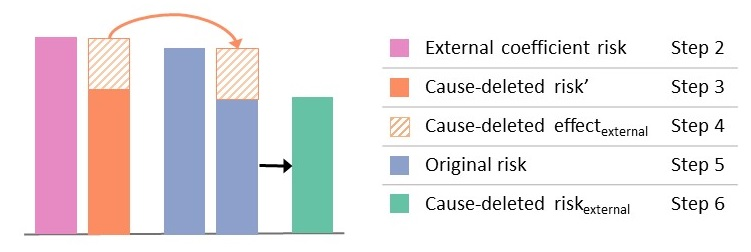
\includegraphics{Images/Method2 only -cbf} 

}

\caption{Risk portion of the health behaviour attribution calculations}\label{fig:unnamed-chunk-26}
\end{figure}

\hypertarget{part-b-health-outcome-calculations}{%
\subsection{Part B: Health outcome calculations}\label{part-b-health-outcome-calculations}}

Using risks generated above you can then calculate:

\begin{itemize}
\tightlist
\item
  Health behaviour-deleted life expectancy or health behaviour attributable life expectancy lost
\item
  Health behaviour-deleted number of deaths or health behaviour attributable number of deaths
\end{itemize}

\textbf{Life expectancy calculations}

Step I: Calculate the original life expectancy by using the original risk (Step 5 above) in the sex-specific 5-year abridge period life tables.

Step II: Calculate the health behaviour-deleted life expectancy by using the health behaviour-deleted risk external (Step 6 above) in the sex-specific 5-year abridge period life tables.

Step III: Calculate the health behaviour attributable life expectancy lost by: original life expectancy (Step I) minus health behaviour-deleted life expectancy (Step II):

\[ \text{Health behaviour attributable life exectancy lost} = \text{Health behaviour-deleted life expectancy} - \text{Original life expectancy}\]

\textbf{Number of deaths calculations}

Step I: Calculate the number of deaths that would occur using the original risk (Step 5 above).

Step II: Calculate the number of deaths that would occur using the health behaviour-deleted risk external (Step 6 above).

Step III: Calculate the health behaviour attributable deaths by: original number of deaths (Step I) minus health behaviour-deleted number of deaths (Step II):

\[\text{Health behaviour attributable deaths} = \text{Original number of deaths} - \text{Health behaviour-deleted number of deaths}\]

\hypertarget{additional-considerations}{%
\section{Additional considerations}\label{additional-considerations}}

\hypertarget{health-behaviours-with-non-monotonic-relationships}{%
\subsection{Health behaviours with non-monotonic relationships}\label{health-behaviours-with-non-monotonic-relationships}}

Health behaviours with relationships that are non-monotonic (always increasing or always decreasing) can be used in health behaviour attributable calculations but special consideration may be warranted for both policy and analytic reasons.

An example of a health behaviour with a non-monotonic relationship is alcohol. Some studies suggest that there is a ``J'' shaped risk relationship for outcomes such as cardiovascular disease.

\emph{Is this still a consideration if we are using 0 as the reference value?}
\emph{Need to complete the thought at the end of the paragraph}
Alcohol drinking guidelines usually do not recommend people: non-drinkers or former-drinkers, initiate drinking. In this situation, the target population for health behaviour attribution calculations can be restricted to for respondents with moderate or higher drinking, or multiple reference exposures could be created.

\hypertarget{health-behaviours-with-interactions-or-multiple-coefficients}{%
\subsection{Health behaviours with interactions or multiple coefficients}\label{health-behaviours-with-interactions-or-multiple-coefficients}}

The health behaviour attributable risk and the health behaviour-deleted risk estimates can be calculated for health behaviours with interaction terms, including complex interactions or multiple coefficients. Examples include:

\begin{itemize}
\tightlist
\item
  health behaviour parametes with age interaction;
\item
  spline functions with terms for each knot point; or,
\item
  composite risks such as smoking which may coefficients for smoking status (current, former, never) and pack-years.
\end{itemize}

All coefficients that related to a common risk factor should be simultaneously considered.

\hypertarget{exposures-not-in-the-original-algorithm}{%
\subsection{Exposures not in the original algorithm}\label{exposures-not-in-the-original-algorithm}}

\hypertarget{licence}{%
\chapter{Licence}\label{licence}}

\emph{Attribution-NonCommercial-ShareAlike 4.0 International}

Creative Commons Corporation (``Creative Commons'') is not a law firm and does not provide legal services or legal advice. Distribution of Creative Commons public licenses does not create a lawyer-client or other relationship. Creative Commons makes its licenses and related information available on an ``as-is'' basis. Creative Commons gives no warranties regarding its licenses, any material licensed under their terms and conditions, or any related information. Creative Commons disclaims all liability for damages resulting from their use to the fullest extent possible.

\hypertarget{using-creative-commons-public-licenses}{%
\subsection{Using Creative Commons Public Licenses}\label{using-creative-commons-public-licenses}}

Creative Commons public licenses provide a standard set of terms and conditions that creators and other rights holders may use to share original works of authorship and other material subject to copyright and certain other rights specified in the public license below. The following considerations are for informational purposes only, are not exhaustive, and do not form part of our licenses.

\begin{itemize}
\item
  \textbf{Considerations for licensors:} Our public licenses are intended for use by those authorized to give the public permission to use material in ways otherwise restricted by copyright and certain other rights. Our licenses are irrevocable. Licensors should read and understand the terms and conditions of the license they choose before applying it. Licensors should also secure all rights necessary before applying our licenses so that the public can reuse the material as expected. Licensors should clearly mark any material not subject to the license. This includes other CC-licensed material, or material used under an exception or limitation to copyright. \href{http://wiki.creativecommons.org/Considerations_for_licensors_and_licensees\#Considerations_for_licensors}{More considerations for licensors}.
\item
  \textbf{Considerations for the public:} By using one of our public licenses, a licensor grants the public permission to use the licensed material under specified terms and conditions. If the licensor's permission is not necessary for any reason--for example, because of any applicable exception or limitation to copyright--then that use is not regulated by the license. Our licenses grant only permissions under copyright and certain other rights that a licensor has authority to grant. Use of the licensed material may still be restricted for other reasons, including because others have copyright or other rights in the material. A licensor may make special requests, such as asking that all changes be marked or described. Although not required by our licenses, you are encouraged to respect those requests where reasonable. \href{http://wiki.creativecommons.org/Considerations_for_licensors_and_licensees\#Considerations_for_licensees}{More considerations for the public}.
\end{itemize}

\hypertarget{creative-commons-attribution-noncommercial-sharealike-4.0-international-public-license}{%
\section{Creative Commons Attribution-NonCommercial-ShareAlike 4.0 International Public License}\label{creative-commons-attribution-noncommercial-sharealike-4.0-international-public-license}}

By exercising the Licensed Rights (defined below), You accept and agree to be bound by the terms and conditions of this Creative Commons Attribution-NonCommercial-ShareAlike 4.0 International Public License (``Public License''). To the extent this Public License may be interpreted as a contract, You are granted the Licensed Rights in consideration of Your acceptance of these terms and conditions, and the Licensor grants You such rights in consideration of benefits the Licensor receives from making the Licensed Material available under these terms and conditions.

\hypertarget{section-1-definitions.}{%
\subsection{Section 1 -- Definitions.}\label{section-1-definitions.}}

\begin{enumerate}
\def\labelenumi{\alph{enumi}.}
\item
  \textbf{Adapted Material} means material subject to Copyright and Similar Rights that is derived from or based upon the Licensed Material and in which the Licensed Material is translated, altered, arranged, transformed, or otherwise modified in a manner requiring permission under the Copyright and Similar Rights held by the Licensor. For purposes of this Public License, where the Licensed Material is a musical work, performance, or sound recording, Adapted Material is always produced where the Licensed Material is synched in timed relation with a moving image.
\item
  \textbf{Adapter's License} means the license You apply to Your Copyright and Similar Rights in Your contributions to Adapted Material in accordance with the terms and conditions of this Public License.
\item
  \textbf{BY-NC-SA Compatible License} means a license listed at \href{http://creativecommons.org/compatiblelicenses}{creativecommons.org/compatiblelicenses}, approved by Creative Commons as essentially the equivalent of this Public License.
\item
  \textbf{Copyright and Similar Rights} means copyright and/or similar rights closely related to copyright including, without limitation, performance, broadcast, sound recording, and Sui Generis Database Rights, without regard to how the rights are labeled or categorized. For purposes of this Public License, the rights specified in Section 2(b)(1)-(2) are not Copyright and Similar Rights.
\item
  \textbf{Effective Technological Measures} means those measures that, in the absence of proper authority, may not be circumvented under laws fulfilling obligations under Article 11 of the WIPO Copyright Treaty adopted on December 20, 1996, and/or similar international agreements.
\item
  \textbf{Exceptions and Limitations} means fair use, fair dealing, and/or any other exception or limitation to Copyright and Similar Rights that applies to Your use of the Licensed Material.
\item
  \textbf{License Elements} means the license attributes listed in the name of a Creative Commons Public License. The License Elements of this Public License are Attribution, NonCommercial, and ShareAlike.
\item
  \textbf{Licensed Material} means the artistic or literary work, database, or other material to which the Licensor applied this Public License.
\item
  \textbf{Licensed Rights} means the rights granted to You subject to the terms and conditions of this Public License, which are limited to all Copyright and Similar Rights that apply to Your use of the Licensed Material and that the Licensor has authority to license.
\item
  \textbf{Licensor} means the individual(s) or entity(ies) granting rights under this Public License.
\item
  \textbf{NonCommercial} means not primarily intended for or directed towards commercial advantage or monetary compensation. For purposes of this Public License, the exchange of the Licensed Material for other material subject to Copyright and Similar Rights by digital file-sharing or similar means is NonCommercial provided there is no payment of monetary compensation in connection with the exchange.
\item
  \textbf{Share} means to provide material to the public by any means or process that requires permission under the Licensed Rights, such as reproduction, public display, public performance, distribution, dissemination, communication, or importation, and to make material available to the public including in ways that members of the public may access the material from a place and at a time individually chosen by them.
\item
  \textbf{Sui Generis Database Rights} means rights other than copyright resulting from Directive 96/9/EC of the European Parliament and of the Council of 11 March 1996 on the legal protection of databases, as amended and/or succeeded, as well as other essentially equivalent rights anywhere in the world.
\item
  \textbf{You} means the individual or entity exercising the Licensed Rights under this Public License. Your has a corresponding meaning.
\end{enumerate}

\hypertarget{section-2-scope.}{%
\subsection{Section 2 -- Scope.}\label{section-2-scope.}}

\begin{enumerate}
\def\labelenumi{\alph{enumi}.}
\item
  \textbf{\emph{License grant.}}

  \begin{enumerate}
  \def\labelenumii{\arabic{enumii}.}
  \item
    Subject to the terms and conditions of this Public License, the Licensor hereby grants You a worldwide, royalty-free, non-sublicensable, non-exclusive, irrevocable license to exercise the Licensed Rights in the Licensed Material to:

    A. reproduce and Share the Licensed Material, in whole or in part, for NonCommercial purposes only; and

    B. produce, reproduce, and Share Adapted Material for NonCommercial purposes only.
  \item
    \textbf{Exceptions and Limitations.} For the avoidance of doubt, where Exceptions and Limitations apply to Your use, this Public License does not apply, and You do not need to comply with its terms and conditions.
  \item
    \textbf{Term.} The term of this Public License is specified in Section 6(a).
  \item
    \textbf{Media and formats; technical modifications allowed.} The Licensor authorizes You to exercise the Licensed Rights in all media and formats whether now known or hereafter created, and to make technical modifications necessary to do so. The Licensor waives and/or agrees not to assert any right or authority to forbid You from making technical modifications necessary to exercise the Licensed Rights, including technical modifications necessary to circumvent Effective Technological Measures. For purposes of this Public License, simply making modifications authorized by this Section 2(a)(4) never produces Adapted Material.
  \item
    \textbf{Downstream recipients.}

    A. \textbf{Offer from the Licensor -- Licensed Material.} Every recipient of the Licensed Material automatically receives an offer from the Licensor to exercise the Licensed Rights under the terms and conditions of this Public License.

    B. \textbf{Additional offer from the Licensor -- Adapted Material.} Every recipient of Adapted Material from You automatically receives an offer from the Licensor to exercise the Licensed Rights in the Adapted Material under the conditions of the Adapter's License You apply.

    C. \textbf{No downstream restrictions.} You may not offer or impose any additional or different terms or conditions on, or apply any Effective Technological Measures to, the Licensed Material if doing so restricts exercise of the Licensed Rights by any recipient of the Licensed Material.
  \item
    \textbf{No endorsement.} Nothing in this Public License constitutes or may be construed as permission to assert or imply that You are, or that Your use of the Licensed Material is, connected with, or sponsored, endorsed, or granted official status by, the Licensor or others designated to receive attribution as provided in Section 3(a)(1)(A)(i).
  \end{enumerate}
\item
  \textbf{\emph{Other rights.}}

  \begin{enumerate}
  \def\labelenumii{\arabic{enumii}.}
  \item
    Moral rights, such as the right of integrity, are not licensed under this Public License, nor are publicity, privacy, and/or other similar personality rights; however, to the extent possible, the Licensor waives and/or agrees not to assert any such rights held by the Licensor to the limited extent necessary to allow You to exercise the Licensed Rights, but not otherwise.
  \item
    Patent and trademark rights are not licensed under this Public License.
  \item
    To the extent possible, the Licensor waives any right to collect royalties from You for the exercise of the Licensed Rights, whether directly or through a collecting society under any voluntary or waivable statutory or compulsory licensing scheme. In all other cases the Licensor expressly reserves any right to collect such royalties, including when the Licensed Material is used other than for NonCommercial purposes.
  \end{enumerate}
\end{enumerate}

\hypertarget{section-3-license-conditions.}{%
\subsection{Section 3 -- License Conditions.}\label{section-3-license-conditions.}}

Your exercise of the Licensed Rights is expressly made subject to the following conditions.

\begin{enumerate}
\def\labelenumi{\alph{enumi}.}
\item
  \textbf{\emph{Attribution.}}

  \begin{enumerate}
  \def\labelenumii{\arabic{enumii}.}
  \item
    If You Share the Licensed Material (including in modified form), You must:

    A. retain the following if it is supplied by the Licensor with the Licensed Material:

    \begin{enumerate}
    \def\labelenumiii{\roman{enumiii}.}
    \item
      identification of the creator(s) of the Licensed Material and any others designated to receive attribution, in any reasonable manner requested by the Licensor (including by pseudonym if designated);
    \item
      a copyright notice;
    \item
      a notice that refers to this Public License;
    \item
      a notice that refers to the disclaimer of warranties;
    \item
      a URI or hyperlink to the Licensed Material to the extent reasonably practicable;
    \end{enumerate}

    B. indicate if You modified the Licensed Material and retain an indication of any previous modifications; and

    C. indicate the Licensed Material is licensed under this Public License, and include the text of, or the URI or hyperlink to, this Public License.
  \item
    You may satisfy the conditions in Section 3(a)(1) in any reasonable manner based on the medium, means, and context in which You Share the Licensed Material. For example, it may be reasonable to satisfy the conditions by providing a URI or hyperlink to a resource that includes the required information.
  \item
    If requested by the Licensor, You must remove any of the information required by Section 3(a)(1)(A) to the extent reasonably practicable.
  \end{enumerate}
\item
  \textbf{\emph{ShareAlike.}}
\end{enumerate}

In addition to the conditions in Section 3(a), if You Share Adapted Material You produce, the following conditions also apply.

\begin{enumerate}
\def\labelenumi{\arabic{enumi}.}
\item
  The Adapter's License You apply must be a Creative Commons license with the same License Elements, this version or later, or a BY-NC-SA Compatible License.
\item
  You must include the text of, or the URI or hyperlink to, the Adapter's License You apply. You may satisfy this condition in any reasonable manner based on the medium, means, and context in which You Share Adapted Material.
\item
  You may not offer or impose any additional or different terms or conditions on, or apply any Effective Technological Measures to, Adapted Material that restrict exercise of the rights granted under the Adapter's License You apply.
\end{enumerate}

\hypertarget{section-4-sui-generis-database-rights.}{%
\subsection{Section 4 -- Sui Generis Database Rights.}\label{section-4-sui-generis-database-rights.}}

Where the Licensed Rights include Sui Generis Database Rights that apply to Your use of the Licensed Material:

\begin{enumerate}
\def\labelenumi{\alph{enumi}.}
\item
  for the avoidance of doubt, Section 2(a)(1) grants You the right to extract, reuse, reproduce, and Share all or a substantial portion of the contents of the database for NonCommercial purposes only;
\item
  if You include all or a substantial portion of the database contents in a database in which You have Sui Generis Database Rights, then the database in which You have Sui Generis Database Rights (but not its individual contents) is Adapted Material, including for purposes of Section 3(b); and
\item
  You must comply with the conditions in Section 3(a) if You Share all or a substantial portion of the contents of the database.
\end{enumerate}

For the avoidance of doubt, this Section 4 supplements and does not replace Your obligations under this Public License where the Licensed Rights include other Copyright and Similar Rights.

\hypertarget{section-5-disclaimer-of-warranties-and-limitation-of-liability.}{%
\subsection{Section 5 -- Disclaimer of Warranties and Limitation of Liability.}\label{section-5-disclaimer-of-warranties-and-limitation-of-liability.}}

\begin{enumerate}
\def\labelenumi{\alph{enumi}.}
\item
  \textbf{Unless otherwise separately undertaken by the Licensor, to the extent possible, the Licensor offers the Licensed Material as-is and as-available, and makes no representations or warranties of any kind concerning the Licensed Material, whether express, implied, statutory, or other. This includes, without limitation, warranties of title, merchantability, fitness for a particular purpose, non-infringement, absence of latent or other defects, accuracy, or the presence or absence of errors, whether or not known or discoverable. Where disclaimers of warranties are not allowed in full or in part, this disclaimer may not apply to You.}
\item
  \textbf{To the extent possible, in no event will the Licensor be liable to You on any legal theory (including, without limitation, negligence) or otherwise for any direct, special, indirect, incidental, consequential, punitive, exemplary, or other losses, costs, expenses, or damages arising out of this Public License or use of the Licensed Material, even if the Licensor has been advised of the possibility of such losses, costs, expenses, or damages. Where a limitation of liability is not allowed in full or in part, this limitation may not apply to You.}
\item
  The disclaimer of warranties and limitation of liability provided above shall be interpreted in a manner that, to the extent possible, most closely approximates an absolute disclaimer and waiver of all liability.
\end{enumerate}

\hypertarget{section-6-term-and-termination.}{%
\subsection{Section 6 -- Term and Termination.}\label{section-6-term-and-termination.}}

\begin{enumerate}
\def\labelenumi{\alph{enumi}.}
\item
  This Public License applies for the term of the Copyright and Similar Rights licensed here. However, if You fail to comply with this Public License, then Your rights under this Public License terminate automatically.
\item
  Where Your right to use the Licensed Material has terminated under Section 6(a), it reinstates:

  \begin{enumerate}
  \def\labelenumii{\arabic{enumii}.}
  \item
    automatically as of the date the violation is cured, provided it is cured within 30 days of Your discovery of the violation; or
  \item
    upon express reinstatement by the Licensor.
  \end{enumerate}

  For the avoidance of doubt, this Section 6(b) does not affect any right the Licensor may have to seek remedies for Your violations of this Public License.
\item
  For the avoidance of doubt, the Licensor may also offer the Licensed Material under separate terms or conditions or stop distributing the Licensed Material at any time; however, doing so will not terminate this Public License.
\item
  Sections 1, 5, 6, 7, and 8 survive termination of this Public License.
\end{enumerate}

\hypertarget{section-7-other-terms-and-conditions.}{%
\subsection{Section 7 -- Other Terms and Conditions.}\label{section-7-other-terms-and-conditions.}}

\begin{enumerate}
\def\labelenumi{\alph{enumi}.}
\item
  The Licensor shall not be bound by any additional or different terms or conditions communicated by You unless expressly agreed.
\item
  Any arrangements, understandings, or agreements regarding the Licensed Material not stated herein are separate from and independent of the terms and conditions of this Public License.
\end{enumerate}

\hypertarget{section-8-interpretation.}{%
\subsection{Section 8 -- Interpretation.}\label{section-8-interpretation.}}

\begin{enumerate}
\def\labelenumi{\alph{enumi}.}
\item
  For the avoidance of doubt, this Public License does not, and shall not be interpreted to, reduce, limit, restrict, or impose conditions on any use of the Licensed Material that could lawfully be made without permission under this Public License.
\item
  To the extent possible, if any provision of this Public License is deemed unenforceable, it shall be automatically reformed to the minimum extent necessary to make it enforceable. If the provision cannot be reformed, it shall be severed from this Public License without affecting the enforceability of the remaining terms and conditions.
\item
  No term or condition of this Public License will be waived and no failure to comply consented to unless expressly agreed to by the Licensor.
\item
  Nothing in this Public License constitutes or may be interpreted as a limitation upon, or waiver of, any privileges and immunities that apply to the Licensor or You, including from the legal processes of any jurisdiction or authority.
\end{enumerate}

\begin{quote}
Creative Commons is not a party to its public licenses. Notwithstanding, Creative Commons may elect to apply one of its public licenses to material it publishes and in those instances will be considered the ``Licensor.'' Except for the limited purpose of indicating that material is shared under a Creative Commons public license or as otherwise permitted by the Creative Commons policies published at \href{http://creativecommons.org/policies}{creativecommons.org/policies}, Creative Commons does not authorize the use of the trademark ``Creative Commons'' or any other trademark or logo of Creative Commons without its prior written consent including, without limitation, in connection with any unauthorized modifications to any of its public licenses or any other arrangements, understandings, or agreements concerning use of licensed material. For the avoidance of doubt, this paragraph does not form part of the public licenses.

Creative Commons may be contacted at creativecommons.org
\end{quote}

\hypertarget{bibilography}{%
\chapter{Bibilography}\label{bibilography}}

\bibliography{./bibliography/book.bib,./packages.bib}


\end{document}
